\chapter{Unitarity and Positivity Bounds in the Axion-Like Particle Effective Field Theory\label{ch:ALP_bounds}}

\begin{flushright}
\small

{\color{chapterpaperrule}\rule{\textwidth}{0.5pt}}

\textit{This chapter is based on Ref.~\cite{Bresciani:2025ojh}:}\\[0.5em]
L.~C.~Bresciani, G.~Levati and P.~Paradisi,\\
``Positivity and partial wave unitarity bounds on ALP theories via amplitude methods,''\\
\href{https://doi.org/10.1007/JHEP07(2026)172}{JHEP \textbf{07} (2026), 172}
%doi.org/10.1007/JHEP07(2026)172
[\href{https://doi.org/10.48550/arXiv.2510.13953}{arXiv:2510.13953} [hep-ph]].

{\color{chapterpaperrule}\rule{\textwidth}{0.5pt}}
\end{flushright}

\section{Introduction}

Axion-like particles (ALPs) were introduced in Chapter~\ref{ch:ALP_RGEs} as light spin-zero bosons
arising in several extensions of the SM as the pseudo-Nambu--Goldstone bosons (pNGBs) of a global
symmetry spontaneously broken at energies much larger than the electroweak
scale~\cite{Jaeckel:2010ni,Marsh:2015xka,Irastorza:2018dyq,DiLuzio:2020wdo}. They generalize the QCD
axion, since their mass and their symmetry-breaking scale are independent parameters to be probed by
experiment. ALPs lighter than the MeV scale can leave their imprints in cosmological and
astrophysical searches, while larger masses are explored at colliders and through a variety of rare
processes~\cite{DiLuzio:2023ndz}. Their interactions with SM fields are conventionally described in a
model-independent way by effective operators, starting at mass dimension five~\cite{Georgi:1986df}.
The complete set of operators invariant under the shift symmetry has been systematically classified
--- up to mass dimension eight --- in Refs.~\cite{Song:2023lxf,Grojean:2023tsd,Bertuzzo:2023slg}, in
part by means of the same on-shell techniques~\cite{DeAngelis:2022qco,Li:2022tec} employed throughout
this thesis.

The pNGB nature of ALPs forbids non-derivative interactions with SM fields. As a result, ALP
amplitudes exhibit an inherent growth with energy, which makes ALP EFTs particularly prone to strong
unitarity constraints and singles them out as a natural arena for the partial-wave unitarity bounds
formulated in Chapter~\ref{ch:generalizedUB}. The energy growth becomes steeper as the dimensionality
of the operator increases, so that the constraints tighten with the mass dimension, while the
expected phenomenological impact of the operator decreases. The two effects do not compensate each
other, and higher-dimensional interactions can dominate physical observables over wide regions of the
parameter space~\cite{Bertuzzo:2023slg}, which is what makes bounds on them worth deriving.

The aim of this chapter is to apply the method of Chapter~\ref{ch:generalizedUB} extensively to ALP
EFTs up to mass dimension eight, improving and generalizing previous results in the literature. We
revisit the bounds of Ref.~\cite{Brivio:2021fog} on the dimension-five operators and extend them to
weak-violating ALP interactions, which exhibit energy enhancements in several processes such as
charged-meson and $W$-boson decays~\cite{Altmannshofer:2022ckw}. We then address the bounds on the
dimension-seven and dimension-eight operators of
Refs.~\cite{Song:2023lxf,Grojean:2023tsd,Bertuzzo:2023slg}.

Finally, we evaluate the complete set of positivity bounds for ALP EFTs and discuss their
complementarity and interplay with the partial-wave unitarity constraints, along the lines of
Chapter~\ref{ch:generalizedUB}. Positivity bounds follow from requiring the EFT to be the low-energy
limit of a unitary, local, and causal quantum field theory~\cite{Adams:2006sv}, as derived in
Section~\ref{sec:analyticity}, and provide a powerful handle on the parameter space of consistent
EFTs. They have been applied across a broad range of frameworks, including the
SMEFT~\cite{Bellazzini:2018paj,Zhang:2020jyn,Bonnefoy:2025uzf,Bi:2019phv,Remmen:2019cyz,%
Remmen:2020vts,Fuks:2020ujk,Yamashita:2020gtt,Gu:2020ldn,Bonnefoy:2020yee,Henriksson:2021ymi,%
Zhang:2021eeo,Chala:2021wpj,Chala:2023jyx,Chala:2023xjy,Li:2022rag,Ghosh:2022qqq,Li:2022aby,%
Gu:2023emi,Chen:2023bhu,Ye:2024rzr,Ye:2025zhs,Davighi:2023acq}, the Higgs
EFT~\cite{Remmen:2024hry,Chakraborty:2024ciu}, and gravitational
theories~\cite{Cheung:2016yqr,Bellazzini:2017fep,deRham:2017xox,Alberte:2020jsk,Hong:2023zgm,%
Alviani:2024sxx,Tokuda:2020mlf,Alberte:2020bdz,Chiang:2022jep,deRham:2022gfe,Caron-Huot:2021rmr,%
Alberte:2021dnj,Caron-Huot:2022ugt}.

The chapter is organized as follows. In Section~\ref{sec:ALPUBeft} we present the ALP EFT, including
effective operators up to mass dimension eight. In Section~\ref{sec:ALPUBunitarity} we systematically
present the partial-wave unitarity bounds in our scenario, emphasizing the important role of a
coupled-channel analysis. In Section~\ref{sec:positivity} we discuss positivity bounds for
dimension-eight operators and their complementarity with partial-wave unitarity bounds.
Section~\ref{sec:ALPUBpheno} is dedicated to some phenomenological applications of our results. Our
conclusions are discussed in Section~\ref{sec:ALPUBconclusions}. Finally, in
Appendix~\ref{app:ALPUBamplitudes} we list the relevant amplitudes to obtain the most stringent
partial-wave unitarity bounds reported in the main text, while in Appendix~\ref{app:UVext} we test
the obtained positivity bounds against a specific ultraviolet extension.

\section{Effective Field Theory for Axion-Like Particles\label{sec:ALPUBeft}}

ALP interactions with SM fields 
are generated starting from dimension-five effective operators \cite{Georgi:1986df}.
The ALP EFT Lagrangian takes the form
\begin{equation}
    \mathcal L_{\phi} = \frac{1}{2}(\partial_\mu \phi) (\partial^\mu \phi) - \frac{1}{2}m_\phi^2 \phi^2 + \sum_{d,k}\coef{d}{k}{}\op{d}{k}{}
\end{equation}
with $d = [\op{d}{k}{}] = 4- [\coef{d}{k}{}]\in\{5,6,7,8\}$.
%
The complete set of operators invariant under a shift symmetry has been systematically classified in \cite{Song:2023lxf,Grojean:2023tsd,Bertuzzo:2023slg} up to mass dimension eight and is reported in Tables \ref{tab:ALPdim5-6}, \ref{tab:ALPdim7}, and \ref{tab:ALPdim8}.

%% DIM 5, 6 %%
\begin{table}[htbp]
\centering
%\begin{adjustbox}{width=1\textwidth,center}
\setlength{\tabcolsep}{1pt}
\renewcommand{\arraystretch}{1.5}
\begin{tabular}{ c|c||c|c||c|c }
\toprule
\multicolumn{2}{c||}{\cellcolor{hdrcolor}\hyperref[par:phipsi2H]{\boldmath$\phi\psi^2 H+\text{\bf H.c.}$}} & \multicolumn{2}{c||}{\cellcolor{hdrcolor}\hyperref[par:phiX2]{\boldmath$\phi X^2$}} & \multicolumn{2}{c}{\cellcolor{hdrcolor}\hyperref[par:phi2H2D2]{\boldmath$\phi^2 H^2 D^2$}} \\
\hline
$\op{5}{\phi \ell e H}{pr}$ & $\phi\, \overline \ell_p  e_r H$ & $\op{5}{\phi B^2}{}$ & $\phi\, B_{\mu\nu}\widetilde B^{\mu\nu}$&$\op{6}{\phi^2 H^2}{}$& $(\partial_\mu \phi\, \partial^\mu \phi)(H^\dagger H)$ 
\\ 
$\op{5}{\phi q u H}{pr}$ & $\phi\, \overline q_p  u_r \widetilde H$ & $\op{5}{\phi W^2}{}$ & $\phi\, W^I_{\mu\nu}\widetilde W^{I \mu\nu}$ &\multicolumn{2}{c}{}
\\
$\op{5}{\phi q d H}{pr}$ & $\phi\, \overline q_p  d_r H$ & $\op{5}{\phi G^2}{}$ & $\phi\, G^A_{\mu\nu}\widetilde G^{A\mu\nu}$ &\multicolumn{2}{c}{}
\\
\bottomrule
\end{tabular}
%\end{adjustbox}
\caption{Dimension-five and -six ALP operators.
Operators with $+ \text{H.c.}$ have Hermitian conjugates.
The indices $p,r$ denote weak eigenstates. The labels of the operator classes contain a cross-reference to the corresponding unitarity bounds.\label{tab:ALPdim5-6}}
\end{table}
%% DIM 7 %%
\begin{table}[h!tb]
\centering
\setlength{\tabcolsep}{1pt}
\renewcommand{\arraystretch}{1.5}
\begin{tabular}{ c|c||c|c }
\toprule
\multicolumn{2}{c||}{\cellcolor{hdrcolor}\hyperref[par:phipsi2XD]{\boldmath$\phi \psi^2 X D$}} & \multicolumn{2}{c}{\cellcolor{hdrcolor}\hyperref[par:phiXH2D2]{\boldmath$\phi X H^2 D^2$}} \\
\hline
$\op{7}{\phi \ell^2 B}{(1)pr}$ & $(\partial^\mu \phi)(\overline \ell_p \gamma^\nu \ell_r)B_{\mu\nu}$ & $\op{7}{\phi B H^2}{(1)}$ & $i(\partial_\mu \phi)(H^\dagger \overset{\leftrightarrow}{D}{}_\nu H)B^{\mu\nu}$
\\
$\op{7}{\phi \ell^2 B}{(2)pr}$ & $(\partial^\mu \phi)(\overline \ell_p \gamma^\nu \ell_r)\widetilde B_{\mu\nu}$  & $\op{7}{\phi B H^2}{(2)}$ & $i(\partial_\mu \phi)(H^\dagger \overset{\leftrightarrow}{D}{}_\nu H) \widetilde B^{\mu\nu}$
\\
$\op{7}{\phi e^2 B}{(1)pr}$ & $(\partial^\mu \phi)(\overline e_p \gamma^\nu e_r)B_{\mu\nu}$ & $\op{7}{\phi W H^2}{(1)}$ & $i(\partial_\mu \phi)(H^\dagger \overset{\leftrightarrow}{D}{}_\nu^I H)W^{I\mu\nu}$
\\
$\op{7}{\phi e^2 B}{(2)pr}$ & $(\partial^\mu \phi)(\overline e_p \gamma^\nu e_r)\widetilde B_{\mu\nu}$  & $\op{7}{\phi W H^2}{(2)}$ & $i(\partial_\mu \phi)(H^\dagger \overset{\leftrightarrow}{D}{}^I_\nu H) \widetilde W^{I\mu\nu}$
\\ \hhline{~|~||--}
$\op{7}{\phi q^2 B}{(1)pr}$ & $(\partial^\mu \phi)(\overline q_p \gamma^\nu q_r)B_{\mu\nu}$ & \multicolumn{2}{c}{\cellcolor{hdrcolor}\hyperref[par:phipsi2H2D]{\boldmath$\phi \psi^2 H^2 D$}} 
\\ \hhline{~|~||--}
$\op{7}{\phi q^2 B}{(2)pr}$ & $(\partial^\mu \phi)(\overline q_p \gamma^\nu q_r)\widetilde B_{\mu\nu}$   & $\op{7}{\phi \ell^2 H^2}{(1)pr}$ & $(\partial_\mu \phi)(\overline \ell_p \gamma^\mu \ell_r)(H^\dagger H)$ 
\\
$\op{7}{\phi u^2 B}{(1)pr}$ & $(\partial^\mu \phi)(\overline u_p \gamma^\nu u_r)B_{\mu\nu}$  & $\op{7}{\phi \ell^2 H^2}{(2)pr}$ & $(\partial_\mu \phi)(\overline \ell_p \gamma^\mu \sigma^I \ell_r)(H^\dagger \sigma^I H)$
\\
$\op{7}{\phi u^2 B}{(2)pr}$ & $(\partial^\mu \phi)(\overline u_p \gamma^\nu u_r)\widetilde B_{\mu\nu}$  & $\op{7}{\phi q^2 H^2}{(1)pr}$ & $(\partial_\mu \phi)(\overline q_p \gamma^\mu q_r)(H^\dagger H)$
\\
$\op{7}{\phi d^2 B}{(1)pr}$ & $(\partial^\mu \phi)(\overline d_p \gamma^\nu d_r)B_{\mu\nu}$ & $\op{7}{\phi q^2 H^2}{(2)pr}$ & $(\partial_\mu \phi)(\overline q_p \gamma^\mu \sigma^I q_r)(H^\dagger \sigma^I H)$
\\
$\op{7}{\phi d^2 B}{(2)pr}$ & $(\partial^\mu \phi)(\overline d_p \gamma^\nu d_r)\widetilde B_{\mu\nu}$  & $\op{7}{\phi e^2 H^2}{pr}$ & $(\partial_\mu \phi)(\overline e_p \gamma^\mu e_r)(H^\dagger H)$
\\
$\op{7}{\phi \ell^2 W}{(1)pr}$ & $(\partial^\mu \phi)(\overline \ell_p \gamma^\nu \sigma^I \ell_r)W^I_{\mu\nu}$ & $\op{7}{\phi u^2 H^2}{pr}$ & $(\partial_\mu \phi)(\overline u_p \gamma^\mu u_r)(H^\dagger H)$
\\
$\op{7}{\phi \ell^2 W}{(2)pr}$ & $(\partial^\mu \phi)(\overline \ell_p \gamma^\nu \sigma^I \ell_r)\widetilde W^I_{\mu\nu}$ & $\op{7}{\phi d^2 H^2}{pr}$ & $(\partial_\mu \phi)(\overline d_p \gamma^\mu d_r)(H^\dagger H)$
\\ \hhline{~|~||--}
$\op{7}{\phi q^2 W}{(1)pr}$ & $(\partial^\mu \phi)(\overline q_p \gamma^\nu \sigma^I q_r)W^I_{\mu\nu}$ & \multicolumn{2}{c}{\cellcolor{hdrcolor}\hyperref[par:phipsi2HD2]{\boldmath$\phi \psi^2 H D^2 + \text{\bf H.c.}$}} 
\\ \hhline{~|~||--}
$\op{7}{\phi q^2 W}{(2)pr}$ & $(\partial^\mu \phi)(\overline q_p \gamma^\nu \sigma^I q_r) \widetilde W^I_{\mu\nu}$ & $\op{7}{\phi \ell e H}{(1)pr}$ & $(\partial_\mu \phi)(\overline \ell_p D^\mu e_r H)$
\\
$\op{7}{\phi q^2 G}{(1)pr}$ & $(\partial^\mu \phi)(\overline q_p \gamma^\nu \lambda^A q_r)G^A_{\mu\nu}$ & $\op{7}{\phi \ell e H}{(2)pr}$ & $(\partial_\mu \phi)(D^\mu \overline \ell_p e_r H)$ 
\\
$\op{7}{\phi q^2 G}{(2)pr}$ & $(\partial^\mu \phi)(\overline q_p \gamma^\nu \lambda^A q_r) \widetilde G^A_{\mu\nu}$ & $\op{7}{\phi qu H}{(1)pr}$ & $(\partial_\mu \phi)(\overline q_p D^\mu u_r \widetilde H)$ 
\\
$\op{7}{\phi u^2 G}{(1)pr}$ & $(\partial^\mu \phi)(\overline u_p \gamma^\nu \lambda^A u_r)G^A_{\mu\nu}$ & $\op{7}{\phi qu H}{(2)pr}$ & $(\partial_\mu \phi)(D^\mu \overline q_p u_r \widetilde H)$ 
\\
$\op{7}{\phi u^2 G}{(2)pr}$ & $(\partial^\mu \phi)(\overline u_p \gamma^\nu \lambda^A u_r)\widetilde G^A_{\mu\nu}$ & $\op{7}{\phi qd H}{(1)pr}$ & $(\partial_\mu \phi)(\overline q_p D^\mu d_r  H)$
\\
$\op{7}{\phi d^2 G}{(1)pr}$ & $(\partial^\mu \phi)(\overline d_p \gamma^\nu \lambda^A d_r)G^A_{\mu\nu}$ & $\op{7}{\phi qd H}{(2)pr}$ & $(\partial_\mu \phi)(D^\mu \overline q_p d_r H)$ 
\\ \hhline{~|~||--}
$\op{7}{\phi d^2 G}{(2)pr}$ & $(\partial^\mu \phi)(\overline d_p \gamma^\nu \lambda^A d_r)\widetilde G^A_{\mu\nu}$ & \multicolumn{2}{c}{\cellcolor{hdrcolor}\hyperref[par:phiH4D2]{\boldmath$\phi H^4 D^2$}} 
\\  \hhline{~|~||--}
\multicolumn{2}{c||}{} & $\op{7}{\phi H^4}{}$ & $i(\partial^\mu \phi) (H^\dagger \overset{\leftrightarrow}{D}{}_\mu H)(H^\dagger H)$
\\ 
\bottomrule
\end{tabular}
\caption{Dimension-seven ALP operators. Operators with $+ \text{H.c.}$ have Hermitian conjugates. The indices $p,r$ denote weak eigenstates.
$\sigma^I$ are the Pauli matrices and $\lambda^A$ are the Gell-Mann matrices. The labels of the operator classes contain a cross-reference to the corresponding unitarity bounds.\label{tab:ALPdim7}}
\end{table}
%% DIM 8 %%
\begin{table}[tb]
\centering
\setlength{\tabcolsep}{1pt}
\renewcommand{\arraystretch}{1.5}
\begin{tabular}{ c|c||c|c }
\toprule
\multicolumn{2}{c||}{\cellcolor{hdrcolor}\hyperref[par:phi2X2D2]{\boldmath$\phi^2 X^2 D^2$}} & \multicolumn{2}{c}{\cellcolor{hdrcolor}\hyperref[par:phi2psi2D3]{\boldmath$\phi^2 \psi^2 D^3$}} 
\\
\hline
$\op{8}{\phi^2 B^2}{(1)}$ & $(\partial^\mu \phi\, \partial_\nu \phi)B_{\mu\rho}B^{\nu \rho}$ & $\op{8}{\phi^2 \ell^2}{pr}$ & $i(\partial_\mu \phi\, \partial_\nu \phi)(\overline \ell_p \gamma^\mu D^\nu \ell_r)$
\\
$\op{8}{\phi^2 B^2}{(2)}$ & $(\partial_\mu \phi \, \partial^\mu \phi)B_{\nu\rho}B^{\nu\rho}$ & $\op{8}{\phi^2 e^2}{pr}$ & $i(\partial_\mu \phi\, \partial_\nu \phi)(\overline e_p \gamma^\mu D^\nu e_r)$ 
\\
$\op{8}{\phi^2 B^2}{(3)}$ & $(\partial_\mu \phi \, \partial^\mu \phi)B_{\nu\rho}\widetilde B^{\nu\rho}$ & $\op{8}{\phi^2 q^2}{pr}$ & $i(\partial_\mu \phi\, \partial_\nu \phi)(\overline q_p \gamma^\mu D^\nu q_r)$
\\ 
$\op{8}{\phi^2 W^2}{(1)}$ & $(\partial^\mu \phi\, \partial_\nu \phi)W_{\mu\rho}^I W^{I \nu \rho}$ & $\op{8}{\phi^2 u^2}{pr}$ & $i(\partial_\mu \phi\, \partial_\nu \phi)(\overline u_p \gamma^\mu D^\nu u_r)$
\\ 
$\op{8}{\phi^2 W^2}{(2)}$ & $(\partial_\mu \phi \, \partial^\mu \phi)W_{\nu\rho}^I W^{I\nu\rho}$ & $\op{8}{\phi^2 d^2}{pr}$ & $i(\partial_\mu \phi\, \partial_\nu \phi)(\overline d_p \gamma^\mu D^\nu d_r)$
\\ \hhline{~|~||--}
$\op{8}{\phi^2 W^2}{(3)}$ & $(\partial_\mu \phi \, \partial^\mu \phi)W_{\nu\rho}^I \widetilde W^{I\nu\rho}$ & \multicolumn{2}{c}{\cellcolor{hdrcolor}\hyperref[par:phi2psi2HD2]{\boldmath$\phi^2 \psi^2 H D^2 + \text{\bf H.c.}$}} 
\\ \hhline{~|~||--}
$\op{8}{\phi^2 G^2}{(1)}$ & $(\partial^\mu \phi\, \partial_\nu \phi)G_{\mu\rho}^A G^{A\nu \rho}$ & $\op{8}{\phi^2 \ell e H}{pr}$ & $(\partial_\mu \phi \, \partial^\mu \phi)(\overline \ell_p e_r H) $ 
\\ 
$\op{8}{\phi^2 G^2}{(2)}$ & $(\partial_\mu \phi \, \partial^\mu \phi)G_{\nu\rho}^A G^{A\nu\rho}$ & $\op{8}{\phi^2 qu H}{pr}$ & $(\partial_\mu \phi \, \partial^\mu \phi)(\overline q_p u_r \widetilde H) $ 
\\
$\op{8}{\phi^2 G^2}{(3)}$ & $(\partial_\mu \phi \, \partial^\mu \phi)G_{\nu\rho}^A \widetilde G^{A\nu\rho}$ & $\op{8}{\phi^2 qd H}{pr}$ & $(\partial_\mu \phi \, \partial^\mu \phi)(\overline q_p d_r H) $
\\ \hline
 \multicolumn{2}{c||}{\cellcolor{hdrcolor}\hyperref[par:phi4D4]{\boldmath$\phi^4 D^4$}} & \multicolumn{2}{c}{\cellcolor{hdrcolor}\hyperref[par:phi2H2D4]{\boldmath$\phi^2 H^2 D^4$}} 
 \\ \hline
$\op{8}{\phi^4}{}$ & $(\partial_\mu \phi \, \partial^\mu \phi)^2$ & $\op{8}{\phi^2 H^2}{(1)}$ & $(\partial_\mu \partial_\nu \phi\, \partial^\mu \partial^\nu \phi)(H^\dagger H)$ 
\\ \hhline{--||~|~}
\multicolumn{2}{c||}{\cellcolor{hdrcolor}\hyperref[par:phi2H4D2]{\boldmath$\phi^2 H^4 D^2$}} & $\op{8}{\phi^2 H^2}{(2)}$ & $(\partial^\mu \phi \, \partial^\nu \phi)(D_\mu H^\dagger D_\nu H)$ 
\\ \hhline{--||~|~}
$\op{8}{\phi^2 H^4}{}$ & $(\partial_\mu \phi \, \partial^\mu \phi)(H^\dagger H)^2$ & \multicolumn{2}{c}{} 
\\ \bottomrule
\end{tabular}
\caption{Dimension-eight ALP operators that conserve lepton and baryon numbers.
Operators with $+ \text{H.c.}$ have Hermitian conjugates.
The indices $p,r$ denote weak eigenstates. The labels of the operator classes contain a cross-reference to the corresponding unitarity bounds.\label{tab:ALPdim8}}
\end{table}

\section{Unitarity Bounds\label{sec:ALPUBunitarity}}

An interesting framework for performing a detailed analysis of unitarity constraints is that of EFTs for ALPs. 
Indeed, the pNGB nature of the ALP forces its interactions with SM fields to be of derivative type and, therefore, to grow with the energy.
As a result, strong unitarity bounds are typically expected~\cite{Brivio:2021fog}.
Clearly, as the dimensionality of an operator increases, the energy growth of the interaction also increases, leading to more stringent unitarity constraints.
However, the larger the dimensionality of an operator, the smaller its expected phenomenological impact on physical observables. 
One could then question the approach itself of putting unitarity bounds on higher-dimensional operators if their effects are somehow expected to be subdominant in any case.
However, this is not necessarily the case, as was shown, for instance, in \cite{Bertuzzo:2023slg} for the production of a Higgs-ALP pair at a lepton collider: the impact of the dimension-seven operators $\partial_\mu \phi \,D^\mu \overline \ell H e$ and $\partial_\mu \phi \,\overline \ell H D_\mu e$ on the total cross section was shown there to be significantly larger than that due to the dimension-five operator $\phi \,\overline{\ell} H e$ in a wide region of the parameter space.

Motivated by these considerations, we stress the possible relevance of placing unitarity constraints on higher-dimensional ALP interactions, which constitute the subject of this section. 

The bounds derived below rest on the on-shell formalism of Chapter~\ref{ch:generalizedUB}, which we
recall here in the form used throughout. Any scattering amplitude $\ket*{\mathcal A_{i\to f}}$
admits the decomposition
\begin{equation}\label{eq:ALP_pwd}
    \ket*{\mathcal A_{i\to f}} = \sum_J a^J_{i\to f}\,\ket*{\mathcal B^J_{i\to f}}
\end{equation}
over a basis $\ket*{\mathcal B^J_{i\to f}}$ of states of definite total angular momentum $J$, whose
elements are fixed by the normalization
\begin{equation}\label{eq:ALP_norm}
    \langle \mathcal B^J_{i\to f}|\mathcal B^{J'}_{i\to f}\rangle = \int \dd\Phi_i \,\dd\Phi_f \, \mathcal B^{J'}_{i\to f} \left(\mathcal B^J_{i\to f}\right)^* = (2J+1)\,\delta^{JJ'}\,,
\end{equation}
with $\dd\Phi_{i,f}$ the phase-space measures of the initial and final states. With this choice, the
partial-wave coefficients $a^J_{i\to f}$ obey
\begin{equation}\label{eq:ALP_unitarity_bounds}
    \abs*{\Re a^J_{i\to i}}\le 1\,,\qquad
    0\le \Im a^J_{i\to i}\le 2\,,\qquad
    \abs*{a^J_{i\to f}}\le 1\,,
\end{equation}
with $i\neq f$,
which are the inequalities imposed in what follows. We refer to
Chapter~\ref{ch:generalizedUB} for the explicit construction of the basis, obtained by diagonalizing
the Pauli--Lubanski operator on a set of independent spinor-helicity monomials, and for the
derivation of Eq.~\eqref{eq:ALP_unitarity_bounds}.

\subsection{Dimension-Five and -Six Operators}

The dimension-five and -six ALP operators are reported in Table~\ref{tab:ALPdim5-6}.

\subsubsection{$\phi X^2$ Class\label{par:phiX2}}

The most stringent partial-wave unitarity bound associated with the interaction of the type $\coef{5}{\phi X^2}{}\,\phi\, X^{\mathscr A\mu\nu}\widetilde X_{\mu\nu}^{\mathscr A}$, where $X_{\mu\nu}^{\mathscr A}$ is the field strength of a generic gauge group $G$, $\widetilde X_{\mu\nu}^{\mathscr A} = \frac{1}{2}\epsilon_{\mu\nu\rho\sigma}X^{\mathscr A \rho\sigma}$ (with $\epsilon^{0123} = 1$), and $\mathscr A\in\{1,\dotsc,d(G)\}$ is an adjoint index, is
%
\begin{equation}\label{eq:phiX2_unibounds}
    \sqrt{s}\abs{\coef{5}{\phi X^2}{}} \le \min\left\{ \sqrt{\frac{4\pi}{2\,d(G)-1}},\sqrt{\frac{8\pi}{1+\sqrt{32\,d(G)+1}}}\right\}
\end{equation}
%
where $d(G)$ is the dimension of $G$.
This bound is derived from the $J=0$ partial-wave coefficients of the amplitudes for $XX \to XX$ and $XX \to \phi \phi$, constructed with a double insertion of the operator $\op{5}{\phi X^2}{} = \phi\, X^{\mathscr A\mu\nu}\widetilde X_{\mu\nu}^{\mathscr A}$; see Appendix~\ref{app:amplitudes5e6} for their expressions.

This implies that the Wilson coefficients associated with the dimension-five bosonic operators in Table~\ref{tab:ALPdim5-6} are subject to the following individual constraints:\footnote{In Ref.~\cite{Brivio:2021fog} it is claimed that, for $\sqrt{s} \geq 260$~GeV, the strongest bound on $\coef{5}{\phi W^2}{}$ arises from the $W^+ W^- \to Z (\gamma) \phi$ processes as they are linearly dependent on $\coef{5}{\phi W^2}{}$ and scale with energy as $s^{3/2}$. By an explicit calculation of the associated scattering amplitudes, both in the broken and unbroken phases of the SM, we find instead a $s^{1/2}$ energy dependence, as it is also manifest by adopting the \textit{equivalent gauge} of~\cite{Wulzer:2013mza}. As a result, the processes $XX \to XX$ and $XX \to \phi \phi$ set the most stringent bound on $\coef{5}{\phi W^2}{}$ at any energy scale.}
%
\begin{align}
    \sqrt{s}\abs{\coef{5}{\phi B^2}{}} &\le \sqrt{\frac{8\pi}{1+\sqrt{33}}} \approx 1.9\,,
    \\
    \sqrt{s}\abs{\coef{5}{\phi W^2}{}} &\le \sqrt{\frac{8\pi}{1+\sqrt{97}}}\approx 1.5\,,
    \\
    \sqrt{s}\abs{\coef{5}{\phi G^2}{}} &\le \sqrt{\frac{4\pi}{15}} \approx 0.92\,.
\end{align}

For example, the bound for $\coef{5}{\phi B^2}{}$ is obtained by considering the scattering matrix
\begin{equation}
    \mathcal A_{i \to f} = 
    \begin{pmatrix}
        -4\,\coef{5}{\phi B^2}{2}\,\frac{\agl{3}{4}^2\sqr{2}{1}}{\agl{1}{2}} & 0 & 8\,\coef{5}{\phi B^2}{2}\,\sqr{2}{1}^2
        \\
        0 & -4\,\coef{5}{\phi B^2}{2}\,\frac{\agl{1}{2}^2\sqr{4}{3}}{\agl{3}{4}} & 8\,\coef{5}{\phi B^2}{2}\,\agl{1}{2}^2
        \\
        8\,\coef{5}{\phi B^2}{2}\,\agl{3}{4}^2 & 8\,\coef{5}{\phi B^2}{2}\,\sqr{4}{3}^2 & 0
    \end{pmatrix}
\end{equation}
where $i,f\in\{B^-B^-,B^+B^+,\phi \phi\}$.
The associated $J=0$ partial-wave scattering matrix, after including the $1/\sqrt{2}$ factor for identical particle pairs in the initial and final states, is
\begin{equation}
    a^0_{i \to f} = \frac{s}{4\pi}\,\coef{5}{\phi B^2}{2}
    \begin{pmatrix}
        -1 & 0 & 2 \\
        0 & -1 & 2 \\
        2 & 2 & 0
    \end{pmatrix}\,,
\end{equation}
whose eigenvalues are $\frac{-s}{8\pi}(1\pm \sqrt{33})\,\coef{5}{\phi B^2}{2}$ and $\frac{-s}{4\pi}\,\coef{5}{\phi B^2}{2}$.
In this case, since the gauge bosons are Abelian, we have $\mathcal A (B^{\pm}B^{\pm} \to B^{\mp}B^{\mp}) = 0$.
On the other hand, if the gauge bosons are non-Abelian, the associated amplitude for the same helicity configuration no longer vanishes and contributes to having $\frac{-s}{4\pi}(2\,d(G)-1)\,\coef{5}{\phi X^2}{2}$ as an eigenvalue, which corresponds to the first term on the right-hand side of Eq.~\eqref{eq:phiX2_unibounds}.

Stronger bounds can be obtained by considering also scattering processes where these three Wilson coefficients are simultaneously non-vanishing.
In fact, in that case, the amplitudes for $BB \to WW$, $WW \to GG$, and $BB \to GG$ are each proportional to the product of the two different Wilson coefficients.
As a result, if we include them, the bounds on $\coef{5}{\phi B^2}{}$, $\coef{5}{\phi W^2}{}$, and $\coef{5}{\phi G^2}{}$ become correlated and more stringent than when considered independently.
The largest eigenvalues of the entire partial-wave scattering matrix with $J=0$ are given by the roots $x_i$ of the cubic and quartic polynomials
\begin{equation}
    p(x) = a_0 + a_1 x+a_2x^2+x^3\,, \qquad
    q(x) = b_0 + b_1 x + b_2 x^2 + b_3 x^3 + x^4\,,
\end{equation}
with
\begin{align}
    a_0 &= 23\, \coef{5}{\phi B^2}{2}\,\coef{5}{\phi W^2}{2}\,\coef{5}{\phi G^2}{2}\,R^6 \,,\\
    a_1&= - \left(17\, \coef{5}{\phi B^2}{2}\,\coef{5}{\phi G^2}{2}+7\,\coef{5}{\phi B^2}{2}\,\coef{5}{\phi W^2}{2}+21\,\coef{5}{\phi W^2}{2}\,\coef{5}{\phi G^2}{2}\right)R^4\,,\\
    a_2&= \left(\coef{5}{\phi B^2}{2} + 5\,\coef{5}{\phi W^2}{2} + 15\,\coef{5}{\phi G^2}{2}\right) R^2\,,
\end{align}
and
\begin{align}
    b_0 &= -8\, \coef{5}{\phi B^2}{2}\,\coef{5}{\phi W^2}{2}\,\coef{5}{\phi G^2}{2} \left(\coef{5}{\phi B^2}{2}+3\,\coef{5}{\phi W^2}{2}+8\,\coef{5}{\phi G^2}{2}\right) R^8\,,
    \\
    b_1 &= 
    \Big(\coef{5}{\phi B^2}{2}\,\coef{5}{\phi W^2}{2}\,\coef{5}{\phi G^2}{2} -8\,\coef{5}{\phi B^2}{4}\,\coef{5}{\phi W^2}{2}
    -24\,\coef{5}{\phi B^2}{2}\,\coef{5}{\phi W^2}{4}
    -8\,\coef{5}{\phi B^2}{4}\,\coef{5}{\phi G^2}{2}
    \nonumber \\&\quad -24\,\coef{5}{\phi W^2}{4}\,\coef{5}{\phi G^2}{2}
    -64\, \coef{5}{\phi B^2}{2}\,\coef{5}{\phi G^2}{4}
    -64\,\coef{5}{\phi W^2}{2}\,\coef{5}{\phi G^2}{4}\Big) \, R^6\,,
    \\
    b_2 &= 
    \left[
    \coef{5}{\phi B^2}{2}\,\coef{5}{\phi W^2}{2}
    +\coef{5}{\phi B^2}{2}\,\coef{5}{\phi G^2}{2}
    +\coef{5}{\phi W^2}{2}\,\coef{5}{\phi G^2}{2} -8\left( \coef{5}{\phi B^2}{4}+3\,\coef{5}{\phi W^2}{4}+8\,\coef{5}{\phi G^2}{4} \right)\right]R^4\,,
    \\
    b_3 &= \left(\coef{5}{\phi B^2}{2} + \coef{5}{\phi W^2}{2} + \coef{5}{\phi G^2}{2}\right)R^2\,,
\end{align}
%
where $R=\sqrt{s/(4\pi)}$.
The corresponding unitarity bounds are then found by imposing $\abs{x_i} \le 1$ on each root.
Using the Jury stability criterion~\cite{Schur1918} (see also \cite{grove2004periodicities}, Theorems 1.4 and 1.5), we can avoid the explicit calculation of the roots of $p(x)$ and $q(x)$. 
In fact, $\abs{x_i} \le 1$ holds for each root of $p(x)$ and $q(x)$ if and only if all the following inequalities are satisfied, respectively:
\begin{align}
\label{eq:PWUB_d5_phiX2}
    \begin{dcases}
        \abs{a_2+a_0} \le 1 + a_1\,,\\
        \abs{a_2 - 3 a_0 } \le 3- a_1\,,\\
        a_0^2 + a_1 - a_0 a_2 \le 1\,,
    \end{dcases}
    &&
    \begin{dcases}
        \abs{b_1 + b_3} \le 1+b_0+b_2\,,\\
        \abs{b_1 - b_3} \le 2(1-b_0)\,,\\
        b_2 - 3 b_0 \le 3\,,\\
        b_1^2 + b_2 + b_0(1+b_0+b_0 b_2+b_3^2) \le 1 + b_0^3 + 2 b_0 b_2 + (1+b_0) b_1 b_3\,.
    \end{dcases}
\end{align}
%
The corresponding plots, where we take the intersection of the two regions (which is equivalent to taking the most stringent bound), are shown in Figure~\ref{fig:d5phiX2}.

\begin{figure}[tb]
    \centering
    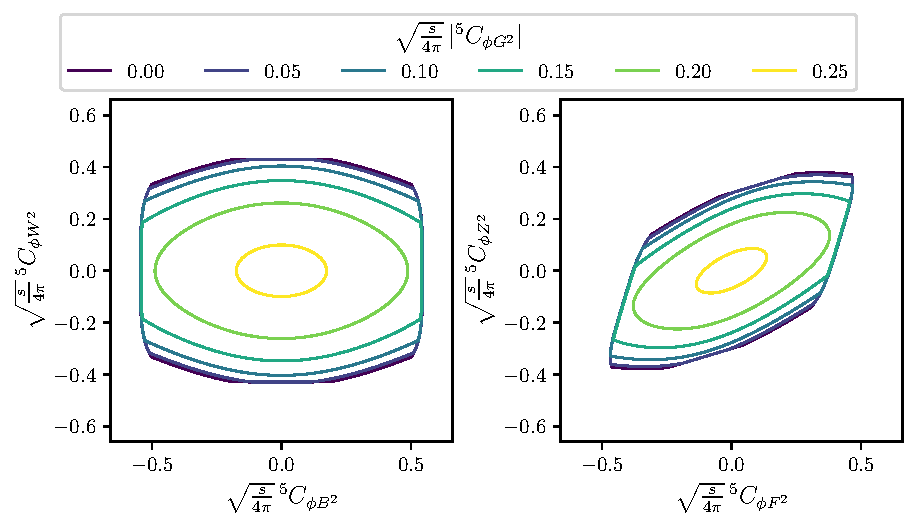
\includegraphics[scale = 0.92]{images/ALPs_d5_phiX2_combined_v2.pdf}
    \caption[Unitarity bounds on the dimension-five axion-like particle couplings to gauge bosons]{Plots of the boundaries of the parameter space allowed by the partial-wave unitarity bounds in Eq.~\eqref{eq:PWUB_d5_phiX2} in the $(\sqrt{s}\,\coef{5}{\phi B^2}{},\sqrt{s}\,\coef{5}{\phi W^2}{})$ plane (left panel) and in the $(\sqrt{s}\,\coef{5}{\phi F^2}{},\sqrt{s}\,\coef{5}{\phi Z^2}{})$ plane (right panel) for different values of $\sqrt{s}\,\abs*{\coef{5}{\phi G^2}{}}$. The Wilson coefficients $\coef{5}{\phi F^2}{}$ and $\coef{5}{\phi Z^2}{}$ are defined as $\coef{5}{\phi F^2}{} = c^2_{\rm W} \, \coef{5}{\phi B^2}{} + s^2_{\rm W}\,\coef{5}{\phi W^2}{}$ and $\coef{5}{\phi Z^2}{} = s^2_{\rm W} \, \coef{5}{\phi B^2}{} + c^2_{\rm W}\,\coef{5}{\phi W^2}{}$ (where $s_{\rm W}$ and $c_{\rm W}$ are the sine and cosine of the weak mixing angle) and mediate the interactions of the ALP with photons and $Z$ bosons, respectively: $\mathcal L \supset \coef{5}{\phi F^2}{} \, \phi \, F_{\mu\nu}\widetilde F^{\mu\nu} + \coef{5}{\phi Z^2}{} \, \phi \, Z_{\mu\nu}\widetilde Z^{\mu\nu}$.}
    \label{fig:d5phiX2}
\end{figure}


\subsubsection{$\phi \psi^2 H$ Class\label{par:phipsi2H}}

The individual bounds for this class of Wilson coefficients are
\begin{gather}
    s \sum_{p,r}\abs{\coef{5}{\phi \ell e H}{pr}}^2 \le 64\pi^2\,,
    \qquad
    s \sum_{p,r}\abs{\coef{5}{\phi qu H}{pr}}^2 \le \frac{64}{3}\pi^2\,,
    \qquad
    s \sum_{p,r}\abs{\coef{5}{\phi qd H}{pr}}^2 \le \frac{64}{3}\pi^2\,,
\end{gather}
while the combined bound is
\begin{equation}
    s \sum_{p,r}\left(\abs{\coef{5}{\phi \ell e H}{pr}}^2 + 3\abs{\coef{5}{\phi qu H}{pr}}^2+3\abs{\coef{5}{\phi qd H}{pr}}^2 \right) \le 64\pi^2\,.
\end{equation}
These are derived from the $J=0$ partial-wave coefficients of the amplitudes for $\phi H \to \psi_p \overline \psi_r$.

\subsubsection{$\phi^2 H^2 D^2$ Class\label{par:phi2H2D2}}

The bound for this Wilson coefficient is
\begin{equation}
    s \abs{\coef{6}{\phi ^2 H^2}{}} \le 8\pi\,,
\end{equation}
which is derived from the $J=0$ partial-wave coefficients of the amplitudes for $\phi \phi \to H\overline H$.

In Figure~\ref{fig:d56summary}, we summarize the marginalized partial-wave unitarity bounds on the Wilson coefficients associated with the dimension-five and -six ALP operators.

\begin{figure}[tb]
    \centering
    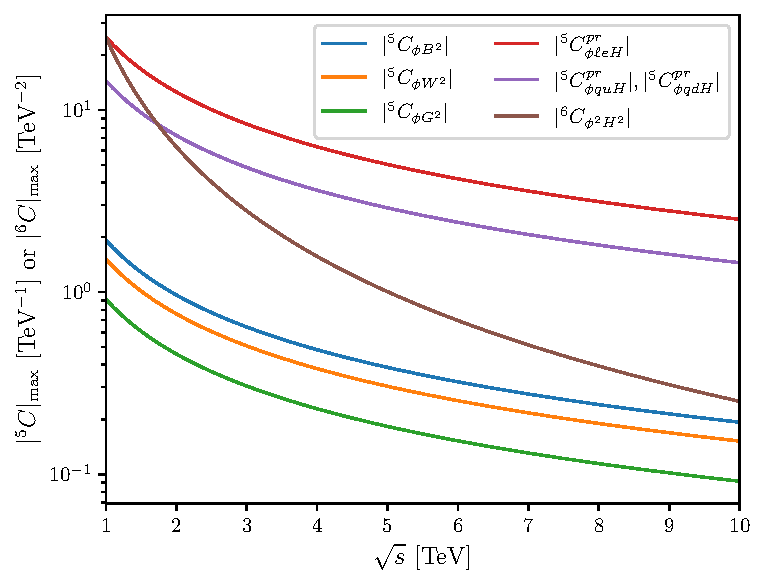
\includegraphics[scale = 0.92]{images/ALPs_d56_summary.pdf}
    \caption[Unitarity bounds on dimension-five and dimension-six axion-like particle operators]{Summary of the marginalized partial-wave unitarity bounds on the Wilson coefficients associated with the dimension-five and -six ALP operators.}
    \label{fig:d56summary}
\end{figure}

\subsection{Dimension-Seven Operators}

The dimension-seven ALP operators are reported in Table~\ref{tab:ALPdim7}.

\subsubsection{$\phi \psi^2 H D^2$ Class\label{par:phipsi2HD2}}

The individual bounds for this class of Wilson coefficients are
\begin{gather}
    s^3 \sum_{p,r}\abs{\coef{7}{\phi \ell e H}{(1)pr} + \coef{7}{\phi \ell e H}{(2)pr}}^2 \le 1024\pi^2\,, \label{eq:PWUB_d7_phipsi2HD2_1}
    \\
    s^{3/2} \abs{3\,\coef{7}{\phi \ell e H}{(1)pr} - \coef{7}{\phi \ell e H}{(2)pr}} \le 96\pi\,,
    \qquad
    s^{3/2} \abs{\coef{7}{\phi \ell e H}{(1)pr} - 3\, \coef{7}{\phi \ell e H}{(2)pr}} \le 96\pi\,,
    \\
    s^3 \sum_{p,r}\abs{\coef{7}{\phi qu H}{(1)pr} + \coef{7}{\phi qu H}{(2)pr}}^2 \le \frac{1024}{3}\pi^2\,,
    \\
    s^{3/2} \abs{3\,\coef{7}{\phi qu H}{(1)pr} - \coef{7}{\phi qu H}{(2)pr}} \le 96\pi\,,
    \qquad
    s^{3/2} \abs{\coef{7}{\phi qu H}{(1)pr} - 3\, \coef{7}{\phi qu H}{(2)pr}} \le 96\pi\,,
    \\
    s^3 \sum_{p,r}\abs{\coef{7}{\phi qd H}{(1)pr} + \coef{7}{\phi qd H}{(2)pr}}^2 \le \frac{1024}{3}\pi^2\,,
    \\
    s^{3/2} \abs{3\,\coef{7}{\phi qd H}{(1)pr} - \coef{7}{\phi qd H}{(2)pr}} \le 96\pi\,,
    \qquad
    s^{3/2} \abs{\coef{7}{\phi qd H}{(1)pr} - 3\, \coef{7}{\phi qd H}{(2)pr}} \le 96\pi\,, \label{eq:PWUB_d7_phipsi2HD2_2}
\end{gather}
while the combined bound is
\begin{equation}
    s^3
    \sum_{p,r}\left(
    \abs{\coef{7}{\phi \ell e H}{(1)pr} + \coef{7}{\phi \ell e H}{(2)pr}}^2
    + 3
    \abs{\coef{7}{\phi qu H}{(1)pr} + \coef{7}{\phi qu H}{(2)pr}}^2
    + 3
    \abs{\coef{7}{\phi qd H}{(1)pr} + \coef{7}{\phi qd H}{(2)pr}}^2
    \right)
     \le 1024\pi^2\,.
\end{equation}
These are derived from the $J=0$ partial-wave coefficients of the amplitudes for $\phi H \to \psi_p \overline \psi_r$ and the $J=1/2$ partial-wave coefficients of the amplitudes for $\phi \psi_p \to H \psi_r$.
The bounds are reported in Figure~\ref{fig:d7phipsi2H}.

\begin{figure}[tb]
    \centering
    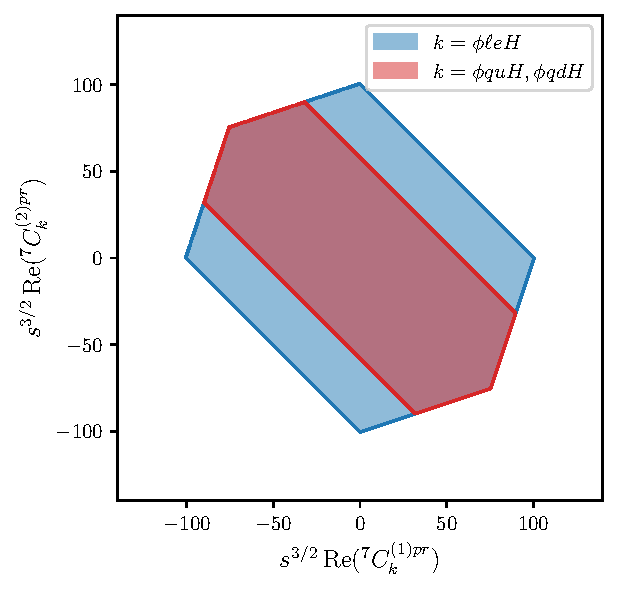
\includegraphics[scale = 0.92]{images/ALPs_d7_phipsi2H.pdf}
    \caption[Unitarity bounds on the dimension-seven axion-like particle operators of the class $\phi\psi^2HD^2$]{Parameter space allowed by partial-wave unitarity bounds in Eqs.~\eqref{eq:PWUB_d7_phipsi2HD2_1}--\eqref{eq:PWUB_d7_phipsi2HD2_2} associated with the dimension-seven operators $\op{7}{k}{(1)pr}$ and $\op{7}{k}{(2)pr}$, with $k=\phi \ell e H,\phi qu H,\phi qd H$ and $p,r=1,2,3$. The imaginary parts of the Wilson coefficients are set to zero.}
    \label{fig:d7phipsi2H}
\end{figure}

\subsubsection{$\phi \psi^2 X D$ Class\label{par:phipsi2XD}}

The bounds for the Wilson coefficients belonging to this class are
%
\begin{align}
    s^{3} \sum_{p,r} \abs{\coef{7}{\phi \ell^2 B}{(1)pr}+ i \,\coef{7}{\phi \ell^2 B}{(2)pr}}^2 &\le 288\pi^2\,,
     &
    s^{3} \sum_{p,r} \abs{\coef{7}{\phi e^2 B}{(1)pr}+ i \,\coef{7}{\phi e^2 B}{(2)pr}}^2 &\le 576\pi^2\,,    
    \\
    s^{3} \sum_{p,r} \abs{\coef{7}{\phi q^2 B}{(1)pr}+ i \,\coef{7}{\phi q^2 B}{(2)pr}}^2 &\le 96 \pi^2\,,
    &
    s^{3} \sum_{p,r} \abs{\coef{7}{\phi u^2 B}{(1)pr}+ i \,\coef{7}{\phi u^2 B}{(2)pr}}^2 &\le 192 \pi^2\,,
    \\
    s^{3} \sum_{p,r} \abs{\coef{7}{\phi d^2 B}{(1)pr}+ i \,\coef{7}{\phi d^2 B}{(2)pr}}^2 &\le 192 \pi^2\,,
    &
    s^{3} \sum_{p,r} \abs{\coef{7}{\phi \ell^2 W}{(1)pr}+ i \,\coef{7}{\phi \ell^2 W}{(2)pr}}^2 &\le 288\pi^2\,,
    \\
    s^{3} \sum_{p,r} \abs{\coef{7}{\phi q^2 W}{(1)pr}+ i \,\coef{7}{\phi q^2 W}{(2)pr}}^2 &\le 96 \pi^2\,,
    &
    s^{3} \sum_{p,r} \abs{\coef{7}{\phi q^2 G}{(1)pr}+ i \,\coef{7}{\phi q^2 G}{(2)pr}}^2 &\le 144 \pi^2\,, 
    \\
    s^{3} \sum_{p,r} \abs{\coef{7}{\phi u^2 G}{(1)pr}+ i \,\coef{7}{\phi u^2 G}{(2)pr}}^2 &\le 288 \pi^2\,,
    & 
    s^{3} \sum_{p,r} \abs{\coef{7}{\phi d^2 G}{(1)pr}+ i \,\coef{7}{\phi d^2 G}{(2)pr}}^2 &\le 288 \pi^2\,.
\end{align}
These are derived from the $J=1$ partial-wave coefficients of the amplitudes for $\phi X \to \psi_p \overline \psi_r$.

\subsubsection{$\phi X H^2 D^2$ Class\label{par:phiXH2D2}}

The bounds for the Wilson coefficients belonging to this class are
\begin{equation}
s^{3/2}\abs{\coef{7}{\phi B H^2}{(1)}+ i \,\coef{7}{\phi B H^2}{(2)}} \le 24\pi\,,
\qquad
s^{3/2}\abs{\coef{7}{\phi W H^2}{(1)}+ i \,\coef{7}{\phi W H^2}{(2)}} \le 24\pi\,.
\end{equation}
These are derived from the $J=1$ partial-wave coefficients of the amplitudes for $\phi X \to H \overline H$.


\subsubsection{$\phi H^4 D^2$ Class\label{par:phiH4D2}}
From the $J=0$ partial-wave coefficients of the amplitudes for $\phi H \to HH\overline H$ we obtain
\begin{equation}
    s^{3/2} \abs{\coef{7}{\phi H^4}{}} \le 16\sqrt{6}\pi^2\,.
\end{equation}

\subsubsection{$\phi \psi^2 H^2 D$ Class\label{par:phipsi2H2D}}
The individual bounds for the Wilson coefficients belonging to this class are
\begin{gather}
    s^3 \sum_{p,r}\abs{\coef{7}{\phi \ell^2 H^2}{(1)pr}}^2 \le (32\sqrt{6}\pi^2)^2 \,,
    \qquad 
    s^3 \sum_{p,r}\abs{\coef{7}{\phi \ell^2 H^2}{(2)pr}}^2 \le (32\sqrt{6}\pi^2)^2 \,,
    \\
    s^3 \sum_{p,r}\abs{\coef{7}{\phi q^2 H^2}{(1)pr}}^2 \le (32\sqrt{2}\pi^2)^2 \,,
    \qquad 
    s^3 \sum_{p,r}\abs{\coef{7}{\phi q^2 H^2}{(2)pr}}^2 \le (32\sqrt{2}\pi^2)^2  \,,
    \\
    s^3 \sum_{p,r}\abs{\coef{7}{\phi e^2 H^2}{pr}}^2 \le (64\sqrt{3}\pi^2)^2 \,,
    \;\,\, 
    s^3 \sum_{p,r}\abs{\coef{7}{\phi u^2 H^2}{pr}}^2 \le (64\pi^2)^2  \,,
    \;\,\,
    s^3 \sum_{p,r}\abs{\coef{7}{\phi d^2 H^2}{pr}}^2 \le (64\pi^2)^2  \,.
\end{gather}
They are derived from the $J=0$ partial-wave coefficients of the amplitudes for $H \overline H \to \phi \psi_p \overline \psi_{r}$.
%
The combined bounds are
\begin{gather}
s^3 \sum_{p,r}\left(\abs{\coef{7}{\phi \ell^2 H^2}{(2)pr}}^2+3\abs{\coef{7}{\phi q^2 H^2}{(2)pr}}^2\right) \le (32\sqrt{6}\pi^2)^2\,,
\\
    s^3 \sum_{p,r}\left(\abs{\coef{7}{\phi e^2 H^2}{pr}}^2 + 3\abs{\coef{7}{\phi u^2 H^2}{pr}}^2+3\abs{\coef{7}{\phi d^2 H^2}{pr}}^2+2\abs{\coef{7}{\phi \ell^2 H^2}{(1)pr}}^2+6\abs{\coef{7}{\phi q^2 H^2}{(1)pr}}^2\right) \le (64\sqrt{3}\pi^2)^2\,.
\end{gather}

In Figure~\ref{fig:d7summary}, we summarize the marginalized partial-wave unitarity bounds on the Wilson coefficients associated with the dimension-seven ALP operators.

\begin{figure}[tb]
    \centering
    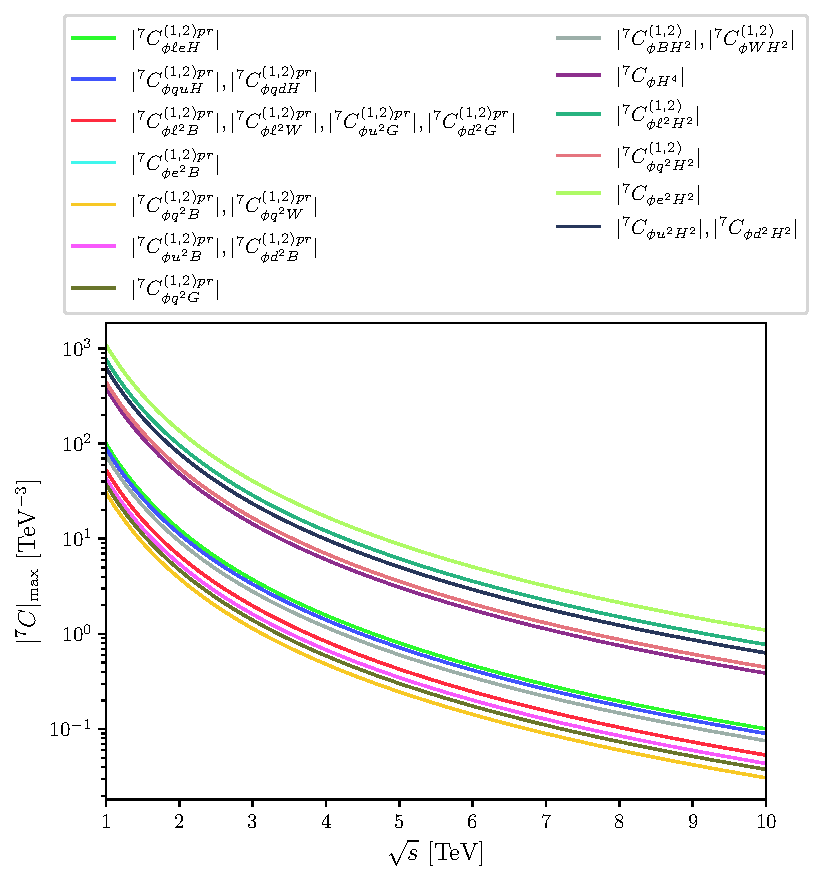
\includegraphics[scale = 0.92]{images/ALPs_d7_summary.pdf}
    \caption[Unitarity bounds on dimension-seven axion-like particle operators]{Summary of the marginalized partial-wave unitarity bounds on the Wilson coefficients associated with the dimension-seven ALP operators.}
    \label{fig:d7summary}
\end{figure}

\subsection{Dimension-Eight Operators}

The dimension-eight ALP operators that conserve lepton and baryon numbers are reported in Table~\ref{tab:ALPdim8}.

\subsubsection{$\phi^4 D^4$ Class\label{par:phi4D4}}
The strongest partial-wave unitarity bound for this Wilson coefficient is
\begin{equation}
    s^2 \abs{\coef{8}{\phi^4}{}} \le \frac{24}{5}\pi
\end{equation}
and is derived from the $J=0$ partial-wave coefficient of the amplitude for $\phi \phi \to \phi \phi$.

\subsubsection{$\phi^2 H^4 D^2$ Class\label{par:phi2H4D2}}
The strongest partial-wave unitarity bound for this Wilson coefficient is
\begin{equation}
    s^2 \abs{\coef{8}{\phi^2 H^4}{}} \le 128\sqrt{2}\pi^3
\end{equation}
and is derived from the $J=0$ partial-wave coefficients of the amplitudes for $\phi \phi \to H\overline HH\overline H$.

\subsubsection{$\phi^2 H^2 D^4$ Class\label{par:phi2H2D4}}
The partial-wave unitarity bounds for this class of Wilson coefficients are
\begin{equation}
    \label{eq:d8-uni_phi2H2}
    s^2 \abs{3\, \coef{8}{\phi^2 H^2}{(1)}+\coef{8}{\phi^2 H^2}{(2)}} \le 48 \pi\,, 
    \qquad 
    s^2  \abs{\coef{8}{\phi^2 H^2}{(1)}+2\, \coef{8}{\phi^2 H^2}{(2)}} \le 48 \pi\,,
\end{equation}
which are derived from the $J=0$ partial-wave coefficients of the amplitudes for $\phi \phi \to H\overline H$ and $\phi H \to \phi H$.
They are shown in Figure~\ref{fig:d8phi2H2}.

\subsubsection{$\phi^2 X^2 D^2$ Class\label{par:phi2X2D2}}
The individual bounds for this class of Wilson coefficients are
\begin{gather}\label{eq:PWUB_d8_phi2X2_1}
s^2 \sqrt{\left(\coef{8}{\phi^2 B^2}{(1)}+4\,\coef{8}{\phi^2 B^2}{(2)}\right)^2+\left(4\,\coef{8}{\phi^2 B^2}{(3)}\right)^2} \le 16 \sqrt{2}\pi\,, \\
s^2 \left[8\abs{\coef{8}{\phi^2 B^2}{(1)}}+3\sqrt{\left(\coef{8}{\phi^2 B^2}{(1)}+4\,\coef{8}{\phi^2 B^2}{(2)}\right)^2+\left(4\,\coef{8}{\phi^2 B^2}{(3)}\right)^2}\right]\le 192 \pi\,,
\\
s^2 \sqrt{\left(\coef{8}{\phi^2 W^2}{(1)}+4\,\coef{8}{\phi^2 W^2}{(2)}\right)^2+\left(4\,\coef{8}{\phi^2 W^2}{(3)}\right)^2} \le 16 \sqrt{\frac{2}{3}}\pi\,, 
\\
s^2 \left[8\abs{\coef{8}{\phi^2 W^2}{(1)}}+3\sqrt{\left(\coef{8}{\phi^2 W^2}{(1)}+4\,\coef{8}{\phi^2 W^2}{(2)}\right)^2+\left(4\,\coef{8}{\phi^2 W^2}{(3)}\right)^2}\right]\le 192 \pi\,,
\\
s^2 \sqrt{\left(\coef{8}{\phi^2 G^2}{(1)}+4\,\coef{8}{\phi^2 G^2}{(2)}\right)^2+\left(4\,\coef{8}{\phi^2 G^2}{(3)}\right)^2} \le 8\pi\,,
\\
s^2 \left[8\abs{\coef{8}{\phi^2 G^2}{(1)}}+3\sqrt{\left(\coef{8}{\phi^2 G^2}{(1)}+4\,\coef{8}{\phi^2 G^2}{(2)}\right)^2+\left(4\,\coef{8}{\phi^2 G^2}{(3)}\right)^2}\right]\le 192 \pi\,,
\label{eq:PWUB_d8_phi2X2_2}
\end{gather}
while the combined one is
\begin{align}
    s^4\bigg[&\left(\coef{8}{\phi^2 B^2}{(1)}+4\,\coef{8}{\phi^2 B^2}{(2)}\right)^2+\left(4\,\coef{8}{\phi^2 B^2}{(3)}\right)^2 + 3 \left(\coef{8}{\phi^2 W^2}{(1)}+4\,\coef{8}{\phi^2 W^2}{(2)}\right)^2+3\left(4\,\coef{8}{\phi^2 W^2}{(3)}\right)^2\nonumber \\
    &+ 8\left(\coef{8}{\phi^2 G^2}{(1)}+4\,\coef{8}{\phi^2 G^2}{(2)}\right)^2+8\left(4\,\coef{8}{\phi^2 G^2}{(3)}\right)^2\bigg]\le (16\sqrt{2}\pi)^2\,.
\end{align}
These bounds are derived from the $J=0$ partial-wave coefficients of the amplitudes for $\phi \phi \to XX$ and the $J=1$ partial-wave coefficients of the amplitudes for $\phi X \to \phi X$.
They are shown in Figure~\ref{fig:d8phi2B2}.

\subsubsection{$\phi^2 \psi^2 D^3$ Class\label{par:phi2psi2D3}}

The strongest individual bounds are
\begin{equation}
    s^2 \abs{\coef{8}{\phi^2 \psi^2}{pr}} \le \frac{96}{5}\pi 
    \qquad
    \text{with~}
    \psi = \ell,e,q,u,d
\end{equation}
and are derived from the $J=1/2$ partial-wave coefficients of the amplitudes for $\phi \psi_p \to \phi \psi_r$.
%
The collective bound is
\begin{equation}
    s^4 \sum_{p,r}\bigg(
    \abs{\coef{8}{\phi^2 e^2}{pr}}^2 
    +2\abs{\coef{8}{\phi^2 \ell^2}{pr}}^2
    + 3 \abs{\coef{8}{\phi^2 u^2}{pr}}^2 
    + 3 \abs{\coef{8}{\phi^2 d^2}{pr}}^2
    + 6 \abs{\coef{8}{\phi^2 q^2}{pr}}^2 
    \bigg) \le (160\sqrt{3}\pi)^2
\end{equation}
and is derived from the $J=2$ partial-wave coefficients of the amplitudes for $\phi \phi \to \psi_p \overline \psi_r$.

\subsubsection{$\phi^2 \psi^2 H D^2$ Class\label{par:phi2psi2HD2}}
The individual bounds for this class of Wilson coefficients are
\begin{gather}
    s^4 \sum_{p,r}\abs{\coef{8}{\phi^2 \ell e H}{pr}}^2 \le (32\sqrt{3}\pi^2)^2\,,\\
    s^4 \sum_{p,r}\abs{\coef{8}{\phi^2 qu H}{pr}}^2 \le (32\pi^2)^2\,,
    \qquad 
    s^4 \sum_{p,r}\abs{\coef{8}{\phi^2 qd H}{pr}}^2 \le (32\pi^2)^2\,.
\end{gather}
%
The combined one is
\begin{equation}
    s^4 \sum_{p,r} \left(\abs{\coef{8}{\phi^2 \ell e H}{pr}}^2 + 3 \abs{\coef{8}{\phi^2 qu H}{pr}}^2 + 3 \abs{\coef{8}{\phi^2 qd H}{pr}}^2\right) \le (32\sqrt{3}\pi^2)^2\,.
\end{equation}
%
These are derived from the $J=0$ partial-wave coefficients of the amplitudes for $\phi \phi \to \psi_p \overline \psi_r H$.

In Figure~\ref{fig:d8summary}, we summarize the marginalized partial-wave unitarity bounds on the Wilson coefficients associated with the dimension-eight ALP operators.

\begin{figure}[tb]
    \centering
    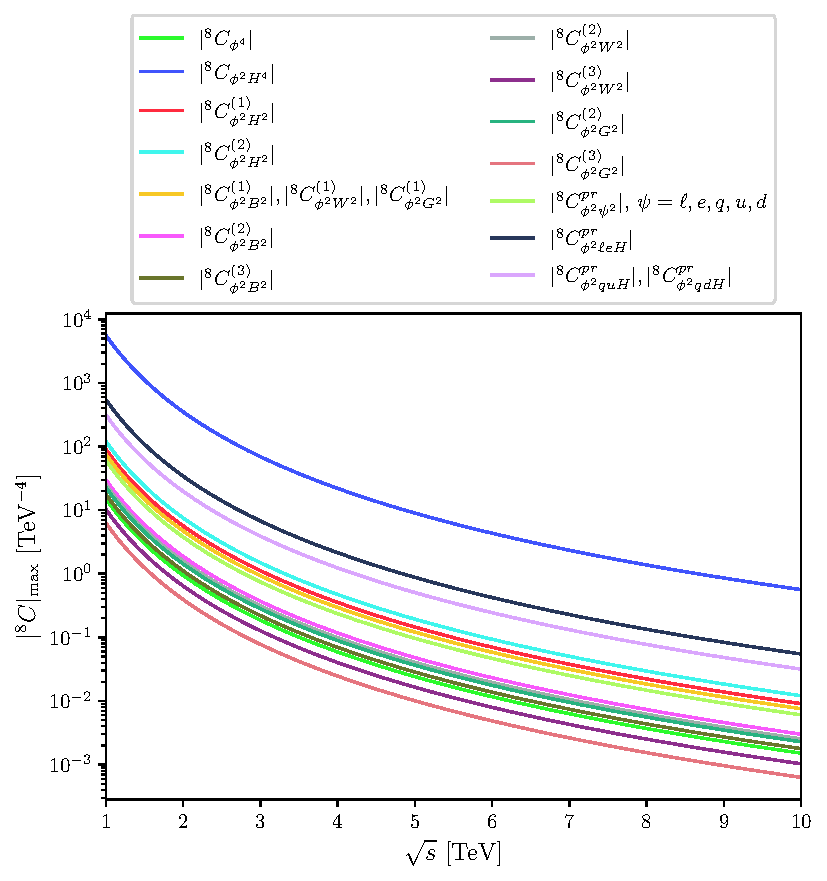
\includegraphics[scale = 0.92]{images/ALPs_d8_summary.pdf}
    \caption[Unitarity bounds on dimension-eight axion-like particle operators]{Summary of the marginalized partial-wave unitarity bounds on the Wilson coefficients associated with the dimension-eight ALP operators.}
    \label{fig:d8summary}
\end{figure}


\subsection{Weak-Violating Axion-Like Particle Interactions with Leptons}
%
The EFT assumed so far was invariant under the electroweak gauge group. If we give up this assumption, ALP-lepton interactions are described by the dimension-five 
Lagrangian~\cite{Altmannshofer:2022ckw}:
%
\begin{equation}
\mathcal{L} = \partial_\mu\phi\, \frac{\overline g_{ll }}{2m_l }\, \overline l  \gamma^\mu l  + \partial_\mu\phi\, \frac{g_{ll}}{2m_l}\, \overline l  \gamma^\mu \gamma_5 l  + \partial_\mu\phi\, \frac{g_{\nu _l }}{2m_l }\, \overline \nu_l \gamma^\mu P_L \nu_l \,,\qquad l = e,\, \mu,\, \tau,
\end{equation} 
%
where the $SU(2)_L$ invariance is recovered for $g_{\nu_l} = \overline g_{ll} - g_{ll}$. The implications of the above interactions are better understood by integrating by parts the Lagrangian~\cite{Altmannshofer:2022ckw}:
%
\begin{align}
-\mathcal{L} &= g_{ll} (\overline l i\gamma_5 l)\, \phi
+ \frac{ e ^2 }{ 16 \pi ^2 m _l } \bigg[ \frac{ \overline{g} _{ll} - 
g _{ll} + g _{\nu_l} }{ 4 s _{\rm W} ^2} W ^+ _{\mu\nu} \widetilde W ^{ {-}\mu \nu } \notag  + \frac{\overline{g} _{ll} - g _{ ll} ( 1 - 4  s _{\rm W} ^2 ) }{ 2 c _{\rm W} s _{\rm W} } F _{\mu\nu} \widetilde{Z} ^{\mu\nu}
\\
&\quad - g _{ll}  F _{\mu\nu} \widetilde{F} ^{\mu\nu} + \notag \frac{ \overline{g} _{ ll} ( 1 - 4 s _{\rm W} ^2 ) - g _{ll} ( 1 - 4 s _{\rm W} ^2 + 8 s _{\rm W} ^4 )  + g _{\nu _l } }{ 8 s _{\rm W} ^2 c _{\rm W} ^2 } Z _{\mu\nu} \widetilde{Z} ^{\mu\nu} \bigg] \,\phi \notag
\\
&\quad + \frac{ig}{2\sqrt{2} m _l }(g_{ll} - \overline g_{ll} + g_{\nu _l }) (\overline l \gamma^\mu P _L \nu_l) W_\mu^- \,\phi + \text{H.c.}\,, 
\label{eq:weak_violating}
\end{align}
%
where $s_{\rm W}$ ($c_{\rm W}$) is the sine (cosine) of the weak mixing angle.
All terms in Eq.~\eqref{eq:weak_violating} are generated 
in the $SU(2)_L$ symmetric limit, except for the last term, which is a genuine electroweak-violating interaction.
As shown in Ref.~\cite{Altmannshofer:2022ckw}, this term generates
an $ ({\rm energy} / m_l )$ enhancement in various processes such as charged meson decays and $W$ boson decays.

The most stringent unitarity bound for the weak-violating combination of coefficients $g_{ll}-\overline g_{ll} + g_{\nu_l}$ is
%
\begin{equation}\label{eq:WV_bounds}
    \frac{s}{m_W m_l}\, g\, \abs{g_{ll}-\overline g_{ll} + g_{\nu_l}} \le 32\sqrt{2}\pi\,,
\end{equation}
%
which is derived from the $J=1/2$ partial-wave coefficient of the amplitude for $\phi l \to W \nu_l$.
In particular, we have the following bounds
%
%
\begin{equation}
    \abs{g_{ll}-\overline g_{ll} + g_{\nu_l}} \lesssim 10^{-5} \left(\frac{m_l}{m_e}\right)
    \left(\frac{\text{TeV}}{\sqrt{s}}\right)^2\,,
\end{equation}
%
which are reported in Figure~\ref{fig:WV}.

\begin{figure}[tb]
    \centering
    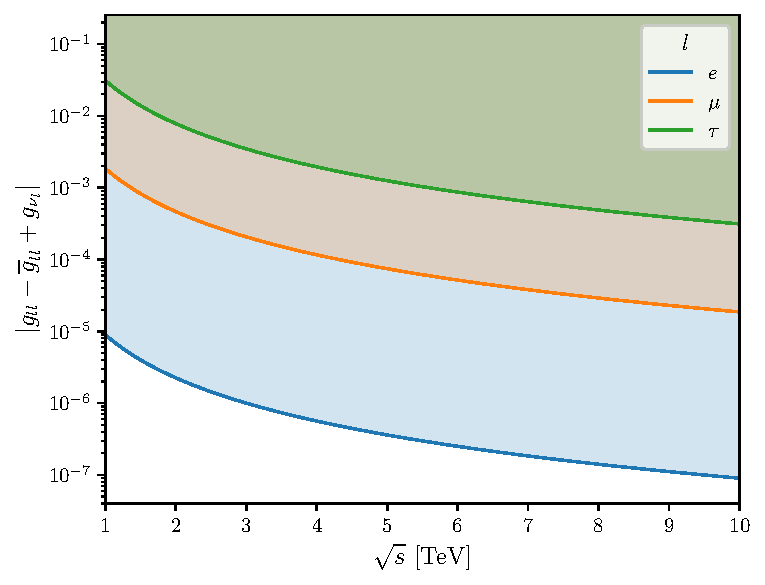
\includegraphics[scale = 0.92]{images/ALPs_WV.pdf}
    \caption[Unitarity bounds on weak-violating axion-like particle couplings to leptons]{Excluded values of the weak-violating combinations $\abs{g_{ll}-\overline{g}_{ll}+g_{\nu_l}}$ as functions of the center-of-mass energy $\sqrt{s}$ by imposing the partial-wave unitarity bounds of Eq.~\eqref{eq:WV_bounds}.}
    \label{fig:WV}
\end{figure}


\section{Positivity Bounds}
\label{sec:positivity}

Positivity bounds, stemming from the requirement that an EFT is the low-energy limit of a unitary, local, and causal quantum field theory~\cite{Adams:2006sv},
provide another set of conditions to infer the viable parameter space of consistent EFTs. 
Hereafter, we evaluate the complete set 
of positivity bounds for ALP EFTs, 
associated with dimension-eight operators,
discussing their complementarity and interplay with partial-wave unitarity constraints~\cite{Bresciani:2025toe}.

Positivity bounds are derived from elastic $2 \to 2$ scattering processes whose amplitudes grow with even powers $n$ of $s$, with $n \ge 2$. 
By considering the scattering of a superposition of states $\ket{u} = \sum_i u_i \ket{i}$ and $\ket{v} = \sum_j v_j \ket{j}$
\begin{equation}
    \mathcal A (s,t) = \mathcal A(u,v \to u,v) = \sum_{i,j,k,l} u_i^* v_j^* u_k v_l \, \mathcal A(i,j\to k,l) \,,
\end{equation}
we can set in the forward limit \cite{Adams:2006sv,Bellazzini:2016xrt}
\begin{equation}
    \left.\dv[2]{}{s} \mathcal A(s,0)\right|_{s=0} \ge 0\,.
\end{equation}

For example, with regard to the operators $\op{8}{\phi^2 H^2}{(1)}$ and $\op{8}{\phi^2 H^2}{(2)}$, if we take 
\begin{equation}
    \ket{u} = \ket{\phi} + x \ket{\pi_a} \,, \qquad \ket{v} = \ket{\phi} + \ket{\pi_a}\,,
\end{equation}
where $\pi_a$ is any of the real components of the Higgs doublet
\begin{equation}
    H =\frac{1}{\sqrt{2}} \begin{pmatrix}
        \pi_1 + i\, \pi_3 \\ \pi_2 + i\, \pi_4 
    \end{pmatrix}\,,
\end{equation}
the amplitude is
\begin{align}
    \mathcal A (s,\theta) &= \mathcal A (u,v \to u,v) \nonumber\\&
    = \frac{s^2}{32}\bigg[
    \coef{8}{\phi^2 H^2}{(1)}\,(6 + 44x + 6x^{2})
  + \coef{8}{\phi^2 H^2}{(2)}\,(11+34x+11x^2)
  \nonumber  \\&\quad - 4 \left(2\,\coef{8}{\phi^2 H^2}{(1)} - \coef{8}{\phi^2 H^2}{(2)}\right)(1 - x)^{2}\cos\theta \nonumber  \\&\quad
  + \left(2\,\coef{8}{\phi^2 H^2}{(1)}\,(1 + x)^{2} + \coef{8}{\phi^2 H^2}{(2)}\,(1+6x+x^2)\right)\cos(2\theta)
\bigg]
\end{align}
and in the forward limit reduces to
\begin{equation}
    \mathcal A (s,0) = \frac{s^2}{2}\left[4\, \coef{8}{\phi^2 H^2}{(1)}\,x +  \coef{8}{\phi^2 H^2}{(2)}\, (1+x)^2\right]\,,
\end{equation}
leading to the bound in Eq.~\eqref{eq:d8-pos_phi2H2} by imposing $4\, \coef{8}{\phi^2 H^2}{(1)}\,x +  \coef{8}{\phi^2 H^2}{(2)} \,(1+x)^2 \ge 0$ for every $x \in \mathbb{R}$.

Another example is provided by the operators $\op{8}{\phi^2 B^2}{(1)}$, $\op{8}{\phi^2 B^2}{(2)}$, and $\op{8}{\phi^2 B^2}{(3)}$.
By parameterizing $\ket{u}$ and $\ket{v}$ as
\begin{equation}
    \ket{u} = \ket{\phi}+x_-\ket{B^-}+x_+\ket{B^+}\,,
    \qquad 
    \ket{v} = \ket{\phi}+y_-\ket{B^-}+y_+\ket{B^+}\,,
\end{equation}
and by using the amplitudes reported in Eqs.~\eqref{eq:ampl_d8_phi2B2(1)} and \eqref{eq:ampl_d8_phi2B2(2)},
the second derivative of $\mathcal A(s,\theta) = \mathcal A(u,v \to u,v)$ with respect to $s$ in the forward limit can be written as
\begin{equation}
    \left.\dv[2]{}{s}\mathcal A(s,0)\right|_{s=0} = \mathbf V\,\mathbf A\,\mathbf V^{T}\,,
\end{equation}
with
\begin{align}
    \mathbf V &=
    \begin{pmatrix}
        \Re x_- & \Im x_- & \Re x_+ & \Im x_+ & \Re y_- & \Im y_- & \Re y_+ & \Im y_+
    \end{pmatrix}\,,
    \\
    \mathbf A &=
    \begin{pmatrix}
-2\,\coef{8}{\phi^2 B^2}{(1)}\,\mathbb{I}_{4} & \mathbf B \\
\mathbf B & -2\,\coef{8}{\phi^2 B^2}{(1)}\,\mathbb{I}_{4}
\end{pmatrix}\,,
\end{align}
and
\begin{equation}
    \mathbf B=
    \begin{pmatrix}
\coef{8}{\phi^2 B^2}{(1)} + 4\,\coef{8}{\phi^2 B^2}{(2)} & -4\,\coef{8}{\phi^2 B^2}{(3)} & \coef{8}{\phi^2 B^2}{(1)} + 4\,\coef{8}{\phi^2 B^2}{(2)} & 4\,\coef{8}{\phi^2 B^2}{(3)} \\
-4\,\coef{8}{\phi^2 B^2}{(3)} & -\coef{8}{\phi^2 B^2}{(1)} - 4\,\coef{8}{\phi^2 B^2}{(2)} & -4\,\coef{8}{\phi^2 B^2}{(3)} & \coef{8}{\phi^2 B^2}{(1)} + 4\,\coef{8}{\phi^2 B^2}{(2)} \\
\coef{8}{\phi^2 B^2}{(1)} + 4\,\coef{8}{\phi^2 B^2}{(2)} & -4\,\coef{8}{\phi^2 B^2}{(3)} & \coef{8}{\phi^2 B^2}{(1)} + 4\,\coef{8}{\phi^2 B^2}{(2)} & 4\,\coef{8}{\phi^2 B^2}{(3)} \\
4\,\coef{8}{\phi^2 B^2}{(3)} & \coef{8}{\phi^2 B^2}{(1)} + 4\,\coef{8}{\phi^2 B^2}{(2)} & 4\,\coef{8}{\phi^2 B^2}{(3)} & -\coef{8}{\phi^2 B^2}{(1)} - 4\,\coef{8}{\phi^2 B^2}{(2)}
\end{pmatrix}\,.
\end{equation}
Finally, by imposing $\mathbf A \succeq 0$, one obtains the constraint in Eq.~\eqref{eq:d8-pos_phi2X2}.

In the following, we present the complete set of positivity bounds associated with the dimension-eight ALP operators listed in Table~\ref{tab:ALPdim8}, and, in Appendix~\ref{app:UVext}, we test them against a specific ultraviolet extension.

\subsubsection{$\phi^4 D^4$ Class}

The positivity bound related to this operator reads~\cite{Ananthanarayan:1994hf,Adams:2006sv}
%
\begin{equation}
    \coef{8}{\phi^4}{} \ge 0\,.
\end{equation}

\subsubsection{$\phi^2 H^2 D^4$ Class}

The positivity bound for this class of Wilson coefficients, 
obtained by considering all possible superpositions of scattering states, is shown in Figure~\ref{fig:d8phi2H2} and reads
\begin{equation}
    \coef{8}{\phi^2 H^2}{(2)}-\abs{2\,\coef{8}{\phi^2 H^2}{(1)}+\coef{8}{\phi^2 H^2}{(2)}} \ge 0\,,
    \label{eq:d8-pos_phi2H2}
\end{equation}
whereas the bound obtained without including such superpositions is
\begin{equation}
    \coef{8}{\phi^2 H^2}{(2)} \ge 0\,.
\end{equation}
They are consistent with those of~\cite{Kim:2023pwf}.

\begin{figure}[tb]
    \centering
    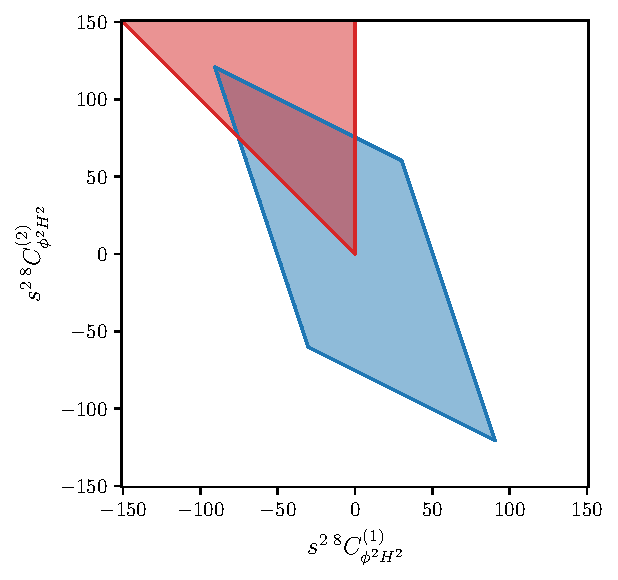
\includegraphics[scale = 0.92]{images/ALPs_d8_phi2H2.pdf}
    \caption[Unitarity and positivity bounds on the dimension-eight class $\phi^2H^2D^4$]{Parameter space allowed by partial-wave unitarity bounds (Eq.~\eqref{eq:d8-uni_phi2H2}, blue) and positivity bounds (Eq.~\eqref{eq:d8-pos_phi2H2}, red) associated with the operators $\op{8}{\phi^2 H^2}{(1)}$ and $\op{8}{\phi^2 H^2}{(2)}$. The intersection area constitutes $1/4$ of the area of the blue region.}
    \label{fig:d8phi2H2}
\end{figure}

\subsubsection{$\phi^2 X^2 D^2$ Class}

The positivity bounds for this class of Wilson coefficients, obtained by considering all possible superpositions of scattering states, are
\begin{equation}
\label{eq:d8-pos_phi2X2}
    \coef{8}{\phi^2 X^2}{(1)} + \sqrt{\left(\coef{8}{\phi^2 X^2}{(1)}+4\,\coef{8}{\phi^2 X^2}{(2)}\right)^2+\left(4\,\coef{8}{\phi^2 X^2}{(3)}\right)^2} \le 0
\end{equation}
for every $X=B,W,G$, and are shown in Figure~\ref{fig:d8phi2B2}, whereas the bounds obtained without including such superpositions are
\begin{equation}
    \coef{8}{\phi^2 X^2}{(1)} \le 0\,.
\end{equation}

\begin{figure}[tb]
    \centering
    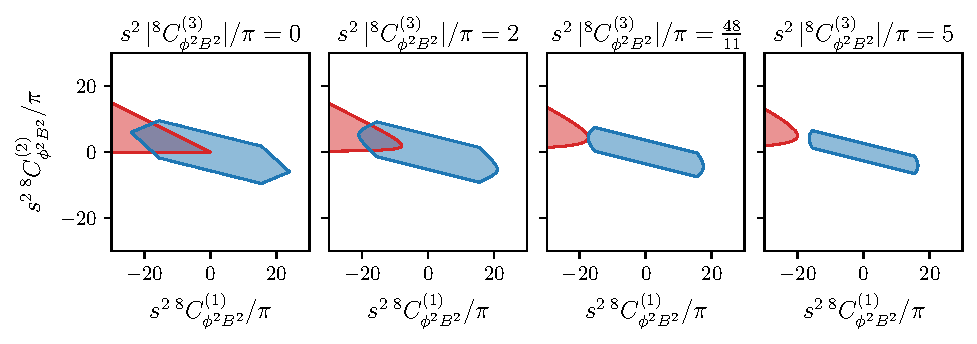
\includegraphics[width=\linewidth]{images/ALPs_d8_phi2B2.pdf}
    \\
    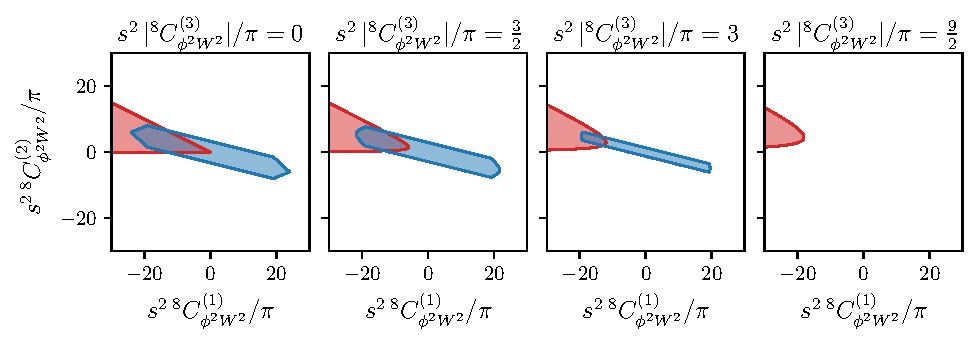
\includegraphics[width=\linewidth]{images/ALPs_d8_phi2W2.pdf}
    \\
    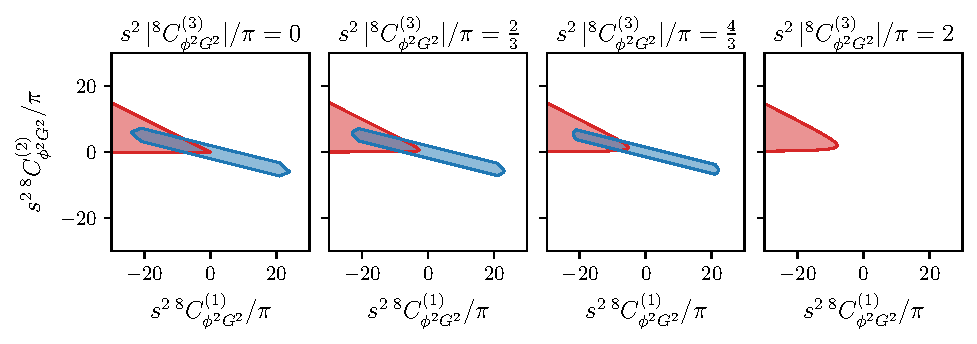
\includegraphics[width=\linewidth]{images/ALPs_d8_phi2G2.pdf}
    \caption[Unitarity and positivity bounds on the dimension-eight class $\phi^2X^2D^2$]{Parameter space allowed by the partial-wave unitarity bounds 
    (Eqs.~\eqref{eq:PWUB_d8_phi2X2_1}--\eqref{eq:PWUB_d8_phi2X2_2}, blue)
    and the positivity constraints 
    (Eq.~\eqref{eq:d8-pos_phi2X2}, red)
    concerning the Wilson coefficients belonging to the class $\phi^2 X^2 D^2$ in the $(s^2\,\coef{8}{\phi^2 X^2}{(1)},s^2\,\coef{8}{\phi^2 X^2}{(2)})$ plane and computed for different values of $s^2\,\abs*{\coef{8}{\phi^2 X^2}{(3)}}$.}
    \label{fig:d8phi2B2}
\end{figure}

To highlight the impact of positivity bounds, we compare the volume of the parameter space allowed by unitarity (see Eqs.~\eqref{eq:PWUB_d8_phi2X2_1}--\eqref{eq:PWUB_d8_phi2X2_2}), $\text{Vol}(\mathscr U)$, with the one obtained after imposing the positivity constraints in Eq.~\eqref{eq:d8-pos_phi2X2}, $\text{Vol}(\mathscr U \cap \mathscr P)$.
In particular, for fixed values of the center-of-mass energy, we find
\begin{equation}
    \frac{\text{Vol}(\mathscr U \cap \mathscr P)}{\text{Vol}(\mathscr U)} = 
    \begin{dcases}
        \frac{36(6+\sqrt{2})}{2057}\approx 0.13 & \text{if~}d(G)=1,\\
        \frac{18\sqrt{d(G)}-11\sqrt{2}}{36\sqrt{d(G)}-6\sqrt{2}} &\text{if~}d(G)\ge 2,
    \end{dcases}
\end{equation}
depending on the dimensionality $d(G)$ of the associated gauge group $G$.

These bounds also apply if we substitute the ALP field with a Higgs doublet.
If one performs this substitution, one finds the dimension-eight SMEFT operators
\begin{align}
    Q^{(1)}_{X^2 H^2 D^2} &= (D^\mu H^\dagger D^\nu H)X^{\mathscr A}_{ \mu\rho}X_\nu^{\mathscr A\rho}\,,
    \\
    Q^{(2)}_{X^2 H^2 D^2} &= (D^\mu H^\dagger D_\mu H)X^{\mathscr A}_{ \nu\rho}X^{\mathscr A \nu \rho}\,,
    \\
    Q^{(3)}_{X^2 H^2 D^2} &= (D^\mu H^\dagger D_\mu H)X^{\mathscr A}_{ \nu\rho}\widetilde X^{\mathscr A \nu \rho}\,,
\end{align}
with $X_{\mu\nu}^{\mathscr A} = B_{\mu\nu},W_{\mu\nu}^I,G_{\mu\nu}^A$, of the basis in \cite{Murphy:2020rsh}.
It follows that the associated Wilson coefficients satisfy the constraints
\begin{equation}
    C_{X^2 H^2 D^2}^{(1)} + \sqrt{\left(C_{X^2 H^2 D^2}^{(1)}+4\,C_{X^2 H^2 D^2}^{(2)}\right)^2+\left(4\,C_{X^2 H^2 D^2}^{(3)}\right)^2} \le 0
\end{equation}
for every $X=B,W,G$,
which represent a generalization of the results presented in \cite{Chala:2023xjy,Remmen:2019cyz} that accounts for a non-vanishing CP-odd $C_{X^2 H^2 D^2}^{(3)}$.

\subsubsection{$\phi^2 \psi^2 D^3$ Class}
The positivity bounds for this class of Wilson coefficients, obtained by considering all possible superpositions of scattering states, are
\begin{equation}
    \coef{8}{\phi^2\psi^2}{} \succeq 0\,,
\end{equation}
or, equivalently,
\begin{align}
\label{eq:pos_d8_phi2psi2_1}
    0\le \Tr (\coef{8}{\phi^2 \psi^2}{}) &= \coef{8}{\phi^2 \psi^2}{11}+\coef{8}{\phi^2 \psi^2}{22}+\coef{8}{\phi^2 \psi^2}{33}\,,
    \\
    0 \le \frac{1}{2}\left[\left(\Tr (\coef{8}{\phi^2 \psi^2}{}) \right)^2 - \Tr (\coef{8}{\phi^2 \psi^2}{2})\right] &= \coef{8}{\phi^2 \psi^2}{11}\,\coef{8}{\phi^2 \psi^2}{22}+\coef{8}{\phi^2 \psi^2}{11}\,\coef{8}{\phi^2 \psi^2}{33}+\coef{8}{\phi^2 \psi^2}{22}\,\coef{8}{\phi^2 \psi^2}{33}\nonumber \\&\quad -\abs{\coef{8}{\phi^2 \psi^2}{12}}^2-\abs{\coef{8}{\phi^2 \psi^2}{13}}^2-\abs{\coef{8}{\phi^2 \psi^2}{23}}^2\,, \label{eq:pos_d8_phi2psi2_2} \\
    0\le \det (\coef{8}{\phi^2 \psi^2}{}) &= \coef{8}{\phi^2 \psi^2}{11}\,\coef{8}{\phi^2 \psi^2}{22}\,\coef{8}{\phi^2 \psi^2}{33}+\coef{8}{\phi^2 \psi^2}{12}\,\coef{8}{\phi^2 \psi^2}{23}\,\coef{8}{\phi^2 \psi^2}{31}\nonumber \\
    &\quad+
    \coef{8}{\phi^2 \psi^2}{13}\,\coef{8}{\phi^2 \psi^2}{32}\,\coef{8}{\phi^2 \psi^2}{21}
    -\coef{8}{\phi^2 \psi^2}{11}\abs{\coef{8}{\phi^2 \psi^2}{23}}^2\nonumber \\
    &\quad-\coef{8}{\phi^2 \psi^2}{22}\abs{\coef{8}{\phi^2 \psi^2}{13}}^2-\coef{8}{\phi^2 \psi^2}{33}\abs{\coef{8}{\phi^2 \psi^2}{12}}^2\,, \label{eq:pos_d8_phi2psi2_3}
\end{align}
for every $\psi = \ell,e,q,u,d$.
This means that:
\begin{itemize}
    \item Every diagonal entry of $\coef{8}{\phi^2 \psi^2}{}$ must be positive;
    \item The modulus of the off-diagonal entries of $\coef{8}{\phi^2 \psi^2}{}$ is bounded from above by combinations of its diagonal entries.
\end{itemize}
Instead, if one did not consider all possible superpositions of scattering states, the resulting bound would just involve the diagonal entries:
\begin{equation}
    \coef{8}{\phi^2 \psi^2}{pp} \ge 0\,.
\end{equation}

Also in this case, by substituting the ALP field with a Higgs doublet, one recovers the dimension-eight SMEFT operators 
\begin{align}
    Q_{\psi^2 H^2 D^3}^{(1)pr} &= i(\overline \psi_p \gamma^\mu D^\nu \psi_r)(D_{(\mu}D_{\nu)} H^\dagger H)\,,
    \\
    Q_{\psi^2 H^2 D^3}^{(2)pr} &= i(\overline \psi_p \gamma^\mu D^\nu \psi_r)(H^\dagger D_{(\mu}D_{\nu)}H)\,,
\end{align}
with $\psi = \ell,e,q,u,d$, of the basis in \cite{Murphy:2020rsh}.
Identifying $\coef{8}{\phi^2\psi^2}{pr}$ with $-\frac{1}{2}C_{\psi^2 H^2 D^3}^{(1)pr}-\frac{1}{2}C_{\psi^2 H^2 D^3}^{(2)pr}$, the positivity bounds in Eqs.~\eqref{eq:pos_d8_phi2psi2_1}--\eqref{eq:pos_d8_phi2psi2_3} are translated in
\begin{equation}\label{eq:pos_smeft_psi2H2D3}
    C^{(1)}_{\psi^2 H^2 D^3} + C^{(2)}_{\psi^2 H^2 D^3} \preceq 0\,,
\end{equation}
or, equivalently,
\begin{align}
    0 &\ge \Tr(C_{\psi^2 H^2 D^3}^{(1)}+C_{\psi^2 H^2 D^3}^{(2)})\,,\\
    0 &\le \left[\Tr(C_{\psi^2 H^2 D^3}^{(1)}+C_{\psi^2 H^2 D^3}^{(2)})\right]^2  - \Tr[\left(C_{\psi^2 H^2 D^3}^{(1)}+C_{\psi^2 H^2 D^3}^{(2)}\right)^2]\,,\\
    0 &\ge\det(C_{\psi^2 H^2 D^3}^{(1)}+C_{\psi^2 H^2 D^3}^{(2)})\,,
\end{align}
for every $\psi = \ell,e,q,u,d$,
which represent a generalization of the results presented in \cite{Chala:2023xjy} that accounts for non-vanishing off-diagonal entries of $C_{\psi^2 H^2 D^3}^{(1)}$ and $C_{\psi^2 H^2 D^3}^{(2)}$.\footnote{According to the results presented in \cite{Chala:2021wpj,Chala:2023jyx,Chala:2023xjy,Liao:2025npz}, one can notice that the positivity bound in Eq.~\eqref{eq:pos_smeft_psi2H2D3} is consistent with the fact that the one-loop renormalization group equation for the combination $C_{\psi^2 H^2 D^3}^{(1)}+C_{\psi^2 H^2 D^3}^{(2)}$, if restricted to the terms stemming from double insertions of dimension-six operators, is positive semidefinite. In fact, from \cite{Bakshi:2024wzz}, we have that, e.g.,
\begin{equation}
    \mu\dv[]{}{\mu}(C_{e^2 H^2 D^3}^{(1)pr}+C_{e^2 H^2 D^3}^{(2)pr}) \supset \frac{1}{4\pi^2} C_{He}^{pq}C_{He}^{qr}\,,
\end{equation}
which is positive semidefinite since $C_{He}$ is a Hermitian matrix, being the Wilson coefficient associated with the operator $Q_{He} = i(H^\dagger \overset{\leftrightarrow}{D}_\mu H)(\overline e \gamma^\mu e)$ \cite{Grzadkowski:2010es}. One can check that the same is true for all the other $\psi$.}

We note that the positivity bounds derived above are obtained at tree level. In the SMEFT context, it is known that one-loop corrections can
quantitatively modify
positivity bounds~\cite{Bellazzini:2020cot,Bellazzini:2021oaj,Chala:2021wpj,Li:2022aby,Ye:2024rzr}. In particular,
renormalization-group running of
the Wilson coefficients induces an energy-scale dependence of the
bounds, while loop
contributions from light states entering the dispersive integral can
shift the resulting
constraints. A systematic inclusion of these effects in the ALP-SMEFT
framework is beyond
the scope of the present work. Nevertheless, the tree-level bounds
derived here provide
the leading-order constraints implied by analyticity, unitarity, and
crossing symmetry.

\section{Phenomenological Applications\label{sec:ALPUBpheno}}

In this section, we provide a few illustrative examples to emphasize the importance of imposing partial-wave unitarity bounds. As we will show, the size of physical effects in several observables can be drastically reduced once we assume perturbative unitarity to hold at a given energy scale.


\subsection{Dimension-Five Couplings to Gauge Bosons}

As a first example, we consider the partial-wave unitarity bounds 
for the dimension-five ALP couplings to gauge bosons. As discussed in Ref.~\cite{Gavela:2019cmq}, non-resonant ALP searches at the LHC
are particularly effective in this case, leading to the excluded 
black regions of Figure~\ref{fig:gaugebosons}.
Depending on the assumed center-of-mass energy $\sqrt{s}$, unitarity bounds can be competitive or superior to the experimental bounds to probe the ALP parameter space. 
%
\begin{figure}[tb]
    \centering
    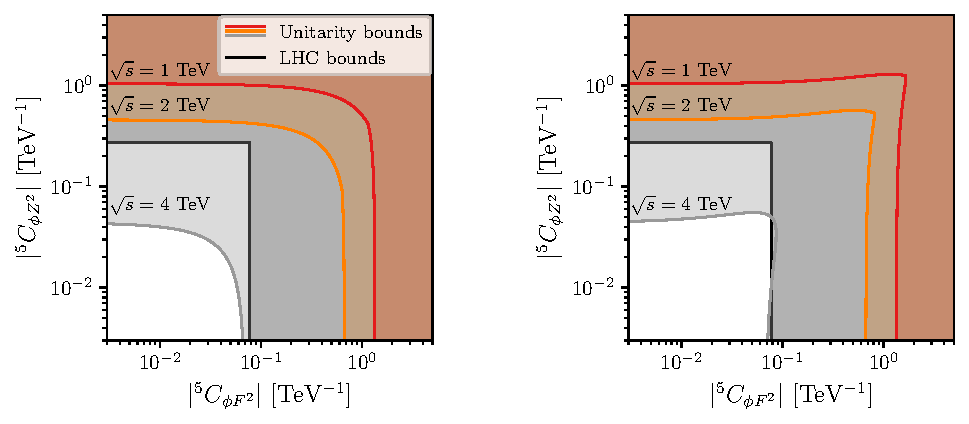
\includegraphics[scale = 0.92]{images/ALPs_gaugebosons.pdf}
    \caption[Unitarity bounds and experimental limits on the axion-like particle couplings to photons and $Z$ bosons]{Parameter space excluded by the partial-wave unitarity bounds in Eq.~\eqref{eq:PWUB_d5_phiX2} for the dimension-five ALP couplings to photons ($\coef{5}{\phi F^2}{} = c^2_{\rm W} \, \coef{5}{\phi B^2}{} + s^2_{\rm W} \,\coef{5}{\phi W^2}{}$) and $Z$ bosons ($\coef{5}{\phi Z^2}{} = s^2_{\rm W} \, \coef{5}{\phi B^2}{} + c^2_{\rm W}\,\coef{5}{\phi W^2}{}$), in the cases where $\coef{5}{\phi F^2}{} \coef{5}{\phi Z^2}{} < 0$ (left panel) and $\coef{5}{\phi F^2}{} \coef{5}{\phi Z^2}{} > 0$ (right panel). In both cases the coupling to gluons has been fixed to $\abs*{\coef{5}{\phi G^2}{}} = 0.225$~TeV$^{-1}$.
    The black region corresponds to the parameter space excluded by Ref.~\cite{Gavela:2019cmq} via non-resonant ALP searches at the LHC, where the limits $\abs*{\coef{5}{\phi F^2}{}\coef{5}{\phi G^2}{}} < 0.018$~TeV$^{-2}$ and $\abs*{\coef{5}{\phi Z^2}{}\coef{5}{\phi G^2}{}} < 0.061$~TeV$^{-2}$ are found for $m_\phi \lesssim 200$~GeV.}
    \label{fig:gaugebosons}
\end{figure}


\subsection{\texorpdfstring{Dimension-Seven Couplings in $l^+ l^- \to \phi h$}{Dimension-Seven Couplings in l+ l- to phi h}}

The relevance of higher-dimensional ALP operators can be nicely illustrated through the process $l^+ l^- \to \phi h$~\cite{Grojean:2023tsd}, which receives contributions from both dimension-five and -seven operators.
In Figure~\ref{fig:crosssection}, we show the cross section for this process in the high-energy limit. The relevant Wilson coefficients are parameterized as $\coef{5}{\phi \ell e H}{ll} = i \, y_l/f$ and $\coef{7}{\phi \ell e H}{(1)ll} = \coef{7}{\phi \ell e H}{(2)ll} = 1/f^3$, where $f$ can be interpreted as the ALP decay constant.

In the high-energy limit, the cross section of $l^+ l^- \to \phi h$ 
is $\sigma = \sigma^{(5)} + \sigma^{(7)}$, where\footnote{The interference term is absent since $\Re{\coef{5}{\phi \ell e H}{ll}\coef{7}{\phi \ell e H}{(1,2)ll}} = 0$ for the benchmark parameterization of the Wilson coefficients.}
%
\begin{equation}
    \sigma^{(7)} = \frac{s^2}{768\pi}\left[\abs{\coef{7}{\phi \ell e H}{(1)ll}}^2+\abs{\coef{7}{\phi \ell e H}{(2)ll}}^2+\Re{\coef{7}{\phi \ell e H}{(1)ll}\,\coef{7}{\phi \ell e H}{(2)ll *}}\right],
\quad
    \sigma^{(5)} = \frac{1}{64\pi}\abs{\coef{5}{\phi \ell e H}{ll}}^2\,.
\end{equation}
%
On the other hand, the partial-wave unitarity bounds lead to the following conditions 
%
\begin{equation}
    \sigma^{(7)} \le \frac{5\pi}{3s}\,,\qquad
    \sigma^{(5)} \le \frac{\pi}{s}\,,
\end{equation}
%
that are illustrated in Figure~\ref{fig:crosssection}.
As a result, large effects to the $l^+ l^- \to \phi h$ cross section can be significantly reduced depending on the ALP decay constant and the center-of-mass energy.
%
\begin{figure}[tb]
    \centering
    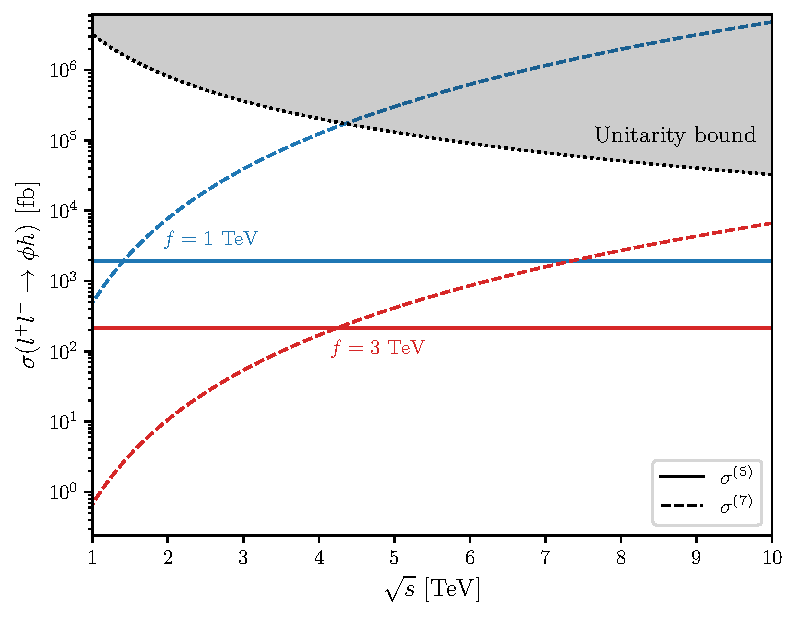
\includegraphics[scale = 0.92]{images/ALPs_crosssection.pdf}
    \caption[High-energy cross section for $l^+l^-\to\phi h$]{Cross section for the process $l^+ l^- \to \phi h$, with $l=e,\mu$, in the high-energy limit. The relevant Wilson coefficients are parameterized as $\coef{5}{\phi \ell e H}{ll} = i \, y_l/f$ and $\coef{7}{\phi \ell e H}{(1)ll} = \coef{7}{\phi \ell e H}{(2)ll} = 1/f^3$, where $f$ can be interpreted as the ALP decay constant.}
    \label{fig:crosssection}
\end{figure}


\subsection{Weak-Violating Axion-Like Particles and Rare Decays}

In the case of weak-violating ALP interacting with electrons (with $\overline g_{ee} = g_{\nu_e} = 0$), the partial-wave unitarity bound reads
%
\begin{equation}
    \abs{g_{ee}} \lesssim 10^{-5} \left(\frac{\text{TeV}}{\sqrt{s}}\right)^2\,.
\end{equation}
%
Instead, in the weak-preserving case (with $\overline g_{ee} = g_{ee}$ and $g_{\nu_e} = 0$), we have
%
\begin{equation}
    \abs{g_{ee}} \lesssim 4 \left(\frac{\text{TeV}}{\sqrt{s}}\right)\,.
\end{equation}

\begin{figure}[tb]
    \centering
    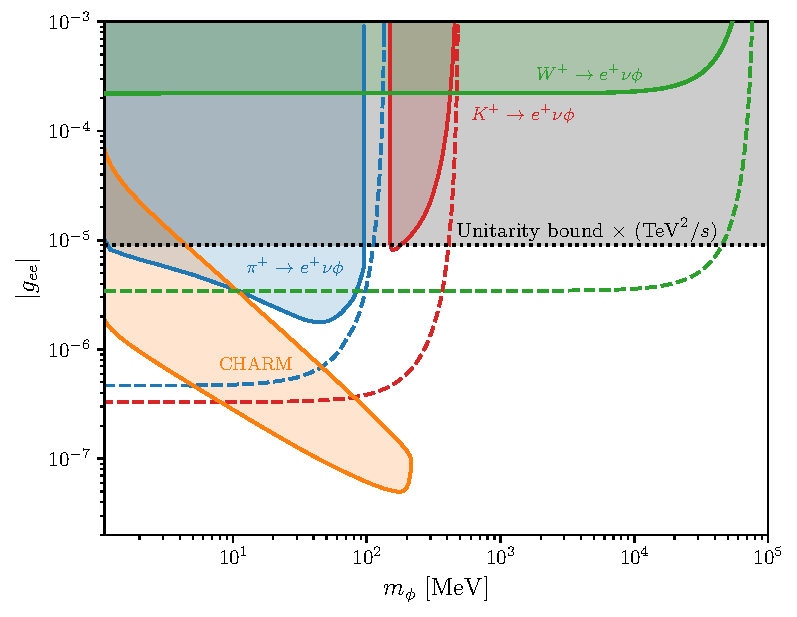
\includegraphics[scale = 0.92]{images/ALPs_WV_gee.pdf}
    \caption[Theoretical and experimental bounds on the weak-violating axion-like particle coupling $g_{ee}$]{Theoretical and experimental bounds on the coupling $g_{ee}$ of a weak-violating ALP~\cite{Altmannshofer:2022ckw}. 
    The partial-wave unitarity bound is shown in grey and scales 
    as $1/s$. 
    Searches for leptonic charged-meson decays are shown in blue (pions)~\cite{PIONEER:2022yag} and red (kaons)~\cite{Poblaguev:2002ug,Altmannshofer:2022ckw}, while searches for rare $W$-boson decays are shown in green~\cite{ParticleDataGroup:2022pth,Altmannshofer:2022ckw}. Bounds from leptonic charged-meson decays in the CHARM proton beam dump~\cite{CHARM:1985anb} are shown in orange~\cite{Altmannshofer:2022ckw}. Dashed lines refer to the potential sensitivities with dedicated searches at the PIONEER experiment~\cite{PIONEER:2022yag} and kaon factories~\cite{Altmannshofer:2022ckw}.}
    \label{fig:WV_gee}
\end{figure}

In order to monitor the impact of the above bounds on physical observables, we consider the branching fractions of $\pi^+\to e^+\nu_e \phi$, $K^+\to e^+\nu_e \phi$, and $W^+\to e^+\nu_e \phi$ decays~\cite{Altmannshofer:2022ckw} in the weak-violating case. 
Neglecting ALP mass effects and taking into account partial-wave unitarity bounds, we find that
%
\begin{align}
    \mathcal B(\pi^+ \to e^+ \nu_e \phi) &\lesssim 4 \times 10^{-9}\left(\frac{\text{TeV}}{\sqrt{s}}\right)^4 \,,
    \\
    \mathcal B(K^+ \to e^+ \nu_e \phi) &\lesssim 7 \times 10^{-8} \left(\frac{\text{TeV}}{\sqrt{s}}\right)^4\,,
    \\
    \mathcal B(W^+ \to e^+ \nu_e \phi) &\lesssim 6 \times 10^{-5} \left(\frac{\text{TeV}}{\sqrt{s}}\right)^4\,.
\end{align}
%
The current bound for the 
$\pi^+ \to e^+ \nu_e \phi$ process arises from the SINDRUM experiment which looked for $e^+e^-$ resonances in $\pi^+ \to e^+ \nu_e \phi$ followed by 
$\phi \to e^+e^-$
with sensitivity to branching ratios of $\mathcal{O}(10^{-10})$~\cite{SINDRUM:1986klz}.
In the future, the PIONEER experiment aims to reach 
the sensitivity of $\mathcal{O}(10^{-11})$~\cite{PIONEER:2022yag}.
Concerning the $K^+ \to e^+ \nu_e \phi$ decay, 
we exploit the E865 search for the SM process 
$K^+ \to e^+ \nu_e e^+e^-$~\cite{Poblaguev:2002ug}. 
Assuming that the ALP channel does not exceed 
twice the uncertainty in this measurement, we impose
the bound $\mathcal{B}(K^+ \to e^+ \nu_e \phi) \leq 4 \times 10^{-9}$~\cite{Altmannshofer:2022ckw}. 
As a future projection, we assume a reference 
bound of $10^{-10}$~\cite{Altmannshofer:2022ckw}.
Moreover, following the analysis of Ref.~\cite{Altmannshofer:2022ckw}, we also impose 
the constraints from leptonic charged meson decays in the CHARM experiment~\cite{CHARM:1985anb}.
As for the $W^+ \to e^+ \nu_e \phi$ decay, we require this mode not to contribute at a visible level to the total width of the $W$ boson
$\Gamma_W = 2.085 \pm 0.042$~GeV~\cite{ParticleDataGroup:2022pth}.
Dedicated analyses for other rare $W$ decays by CMS could improve the bound on the branching ratios of $W^+ \to e^+ \nu_e \phi$ at the level of $10^{-6}$~\cite{Altmannshofer:2022ckw}.

As shown in Figure~\ref{fig:WV_gee}, unitarity bounds already exclude large regions of the parameter space for $\sqrt{s} = 1$~TeV and are typically stronger than the current experimental bounds on charged meson as well as $W$ boson decays.

\section{Conclusions\label{sec:ALPUBconclusions}}

Axion-like particles (ALPs) are generic pseudo-Nambu--Goldstone bosons (pNGBs) emerging from the spontaneous breaking of some global symmetry 
above the electroweak scale. The pNGB nature of ALPs forces their interactions with Standard Model fields to be derivative. Therefore, ALP interactions exhibit an inherent growth with the energy, possibly leading to the breakdown of perturbative unitarity at some large energy scale. 

In this chapter, we have systematically evaluated the partial-wave unitarity bounds for ALP Effective Field Theories (EFTs) including higher-dimensional operators up to dimension eight. The adopted methodology is based on the recently developed formalism described in Chapter~\ref{ch:generalizedUB}, based on on-shell methods, which has proven particularly efficient for studying unitarity bounds of EFTs at high energies~\cite{Bresciani:2025toe}.

In particular, we first revisited and improved the bounds of Ref.~\cite{Brivio:2021fog} relative to dimension-five and -six operators, finding that the processes $XX \to XX$ and $XX \to \phi \phi$ (with $X=B,W,G$) set the most stringent bounds at any energy scale.
The summary of the partial-wave unitarity bounds on the individual
Wilson coefficients associated with these operators is reported in 
Figure~\ref{fig:d56summary}.
Stronger bounds can be obtained through a coupled-channel analysis, 
where several scattering processes such as $BB \to WW$, $WW \to GG$, 
and $BB \to GG$ are generated by the simultaneous presence of different
Wilson coefficients; see Figure~\ref{fig:d5phiX2}.
As a relevant phenomenological application, we discussed the 
impact of the above bounds on non-resonant ALP searches at the LHC~\cite{Gavela:2019cmq}. Unitarity bounds can be competitive or even more stringent than the experimental bounds already for center-of-mass energies at the TeV scale; see Figure~\ref{fig:gaugebosons}. 

Moreover, we discussed partial wave unitarity bounds for dimension-five 
weak-violating ALP interactions; see Figure~\ref{fig:WV}. In this 
case there is a striking energy enhancement $({\rm energy}/m_l)$ 
in several processes such as charged-meson and $W$-boson decays~\cite{Altmannshofer:2022ckw}.
As shown in Figure~\ref{fig:WV_gee}, unitarity bounds exclude large regions of the parameter space already for $\sqrt{s} = 1$~TeV and 
are typically stronger than the current experimental bounds.

Finally, we analyzed the partial-wave unitarity bounds for dimension-seven and -eight operators, which were recently classified in Refs.~\cite{Song:2023lxf,Grojean:2023tsd,Bertuzzo:2023slg}; see
Figures~\ref{fig:d7phipsi2H}, \ref{fig:d7summary}, and \ref{fig:d8summary}.
As a phenomenological application, we considered the process $l^+ l^- \to \phi h$, which receives contributions from both dimension-five and -seven operators, and which can be looked for at future high-energy lepton colliders~\cite{Grojean:2023tsd}. As shown in Figure~\ref{fig:crosssection}, potentially large effects induced by dimension-seven operators are severely reduced depending on the ALP decay constant and the center-of-mass energy.

The last part of this chapter was devoted to the derivation of positivity bounds, stemming from the analyticity and causality of scattering amplitudes, for dimension-eight operators. These were derived from elastic $2 \to 2$ scattering processes that grow with energy as $s^2$.
As shown in Figures~\ref{fig:d8phi2H2} and \ref{fig:d8phi2B2}, positivity and partial-wave unitarity bounds are highly complementary in constraining the parameter space of ALP EFTs. 
Interestingly, our results can also be used to derive new positivity constraints in the SMEFT; see Section~\ref{sec:positivity}.

To conclude, the positivity and partial-wave unitarity bounds derived in this chapter can be applied in several directions, such as ALP searches at colliders, a variety of rare decays, or even as constraints for the event generation, which can impact the shapes of the expected distributions of experimental searches. 
Our work highlights the synergy and interplay of first-principle-based theoretical bounds and experimental limits in our adventure to discover new-physics phenomena.

\begin{subappendices}
    \section{Amplitudes\label{app:ALPUBamplitudes}}

In this appendix we list the relevant amplitudes considered for obtaining the most stringent partial-wave unitarity bounds for the ALP EFT reported in Section~\ref{sec:ALPUBunitarity}.
%
All particles are considered outgoing and massless, since we are interested in the high-energy limit, and the superscripts $\pm$ denote the signs of helicities. 
%
The following notation is used: 
\begin{itemize}
    \item $p,r,\dotsc\in\{1,2,3\}$ are weak-eigenstate indices;
    \item $i,j,\dotsc\in\{1,2\}$ are $SU(2)$ fundamental indices;
    \item $I,J,\dotsc \in \{1,2,3\}$ are $SU(2)$ adjoint indices;
    \item $\alpha,\beta,\dotsc \in\{1,2,3\}$ are $SU(3)$ fundamental indices;
    \item $A,B,\dotsc \in \{1,\dotsc,8\}$ are $SU(3)$ adjoint indices.
\end{itemize}

\subsection{Dimension-Five and -Six Interactions\label{app:amplitudes5e6}}

The relevant amplitudes generated by one or two insertions of dimension-five operators (see Table~\ref{tab:ALPdim5-6}) are 
\begin{align}
\mathcal A(\phi,\ell^-_{ip},\overline e^-_{r},\overline H_j) &= \coef{5}{\phi \ell e H}{pr} \,\agl{2}{3}\delta_{ij} \,, 
\\
\mathcal A(\phi,q^-_{\alpha ip},\overline d^-_{\beta r},\overline H_j) &= \coef{5}{\phi qd H}{pr} \,\agl{2}{3}\delta_{\alpha\beta}\delta_{ij}\,, 
\\
\mathcal A(\phi,q^-_{\alpha ip},\overline u^-_{\beta r}, H_j) &= \coef{5}{\phi qu H}{pr} \,\agl{2}{3}\delta_{\alpha\beta}\epsilon_{ij}\,, 
\\
    \mathcal A(B^+,B^+,B^-,B^-) &= - 4\, \coef{5}{\phi B^2}{2}\,\frac{\agl{3}{4}^2 \sqr{2}{1}}{\agl{1}{2}}\,,  
    \\
    \mathcal A(\phi,\phi,B^-,B^-) &= 8\,\coef{5}{\phi B^2}{2}\,\agl{3}{4}^2\,,
    \\
    \mathcal A(W_I^+,W_J^+,W_K^-,W_L^-) &= - 4\, \coef{5}{\phi W^2}{2}\,\frac{\agl{3}{4}^2 \sqr{2}{1}}{\agl{1}{2}}\delta^{IJ}\delta^{KL}\,, 
    \\
    \mathcal A(W_I^+,W_J^+,W_K^+,W_L^+) &= 4\, \coef{5}{\phi W^2}{2} \bigg[\frac{\sqr{2}{1}\sqr{4}{3}^2}{\agl{1}{2}}\delta^{IJ}\delta^{KL}+\frac{\sqr{3}{1}\sqr{4}{2}^2}{\agl{1}{3}}\delta^{IK}\delta^{JL}\nonumber \\&\quad +\frac{\sqr{4}{1}\sqr{3}{2}^2}{\agl{1}{4}}\delta^{IL}\delta^{JK}\bigg]\,, 
    \\
    \mathcal A(\phi,\phi,W_I^-,W_J^-) &= 8\,\coef{5}{\phi W^2}{2}\,\agl{3}{4}^2 \delta^{IJ}\,,
    \\
    \mathcal A(G_A^+,G_B^+,G_C^-,G_D^-) &= - 4\, \coef{5}{\phi G^2}{2}\,\frac{\agl{3}{4}^2 \sqr{2}{1}}{\agl{1}{2}}\delta^{AB}\delta^{CD}\,, 
    \\
    \mathcal A(G_A^+,G_B^+,G_C^+,G_D^+) &= 4\, \coef{5}{\phi G^2}{2} \bigg[\frac{\sqr{2}{1}\sqr{4}{3}^2}{\agl{1}{2}}\delta^{AB}\delta^{CD}+\frac{\sqr{3}{1}\sqr{4}{2}^2}{\agl{1}{3}}\delta^{AC}\delta^{BD}\nonumber \\&\quad+\frac{\sqr{4}{1}\sqr{3}{2}^2}{\agl{1}{4}}\delta^{AD}\delta^{BC}\bigg] \,, 
    \\
    \mathcal A(\phi,\phi,G_A^-,G_B^-) &= 8\,\coef{5}{\phi G^2}{2}\,\agl{3}{4}^2 \delta^{AB}\,,
    \\
    \mathcal A(B^+,B^+,W_I^-,W_J^-) &= - 4\, \coef{5}{\phi B^2}{}\coef{5}{\phi W^2}{}\,\frac{\agl{3}{4}^2 \sqr{2}{1}}{\agl{1}{2}}\delta^{IJ} \,, 
    \\
    \mathcal A(B^+,B^+,W_I^+,W_J^+) &=  4\, \coef{5}{\phi B^2}{}\coef{5}{\phi W^2}{}\,\frac{\sqr{4}{3}^2 \sqr{2}{1}}{\agl{1}{2}}\delta^{IJ} \,, 
    \\
    \mathcal A(B^+,B^+,G_A^-,G_B^-) &= - 4\, \coef{5}{\phi B^2}{}\coef{5}{\phi G^2}{}\,\frac{\agl{3}{4}^2 \sqr{2}{1}}{\agl{1}{2}}\delta^{AB} \,, 
    \\
    \mathcal A(B^+,B^+,G_A^+,G_B^+) &=  4\, \coef{5}{\phi B^2}{}\coef{5}{\phi G^2}{}\,\frac{\sqr{4}{3}^2 \sqr{2}{1}}{\agl{1}{2}}\delta^{AB} \,, 
    \\
    \mathcal A(W_I^+,W_J^+,G_A^-,G_B^-) &= - 4\, \coef{5}{\phi W^2}{}\coef{5}{\phi G^2}{}\,\frac{\agl{3}{4}^2 \sqr{2}{1}}{\agl{1}{2}}\delta^{IJ}\delta^{AB} \,, 
    \\
    \mathcal A(W_I^+,W_J^+,G_A^+,G_B^+) &=  4\, \coef{5}{\phi W^2}{}\coef{5}{\phi G^2}{}\,\frac{\sqr{4}{3}^2 \sqr{2}{1}}{\agl{1}{2}}\delta^{IJ}\delta^{AB}\,.
\end{align}

The relevant amplitude generated by the only dimension-six operator (see Table~\ref{tab:ALPdim5-6}) is 
\begin{equation}
    \mathcal A(\phi,\phi,H_i,\overline H_j) = -\coef{6}{\phi^2 H^2}{} \,\agl{1}{2}\sqr{2}{1}\delta_{ij}\,.
\end{equation}

\subsection{Dimension-Seven Interactions}

The relevant amplitudes generated by one insertion of dimension-seven operators (see Table~\ref{tab:ALPdim7}) are 
\begin{align}
    \mathcal A(\phi,\ell^-_{ip},\overline e_r^-,\overline H_j)&=-\frac{1}{2}\left(\coef{7}{\phi \ell e H}{(1)pr} \, \agl{1}{3}\sqr{3}{1} + \coef{7}{\phi \ell e H}{(2)pr} \, \agl{1}{2}\sqr{2}{1}\right)\agl{2}{3}\delta_{ij}\,,
    \\
    \mathcal A(\phi,q^-_{\alpha ip},\overline d_{\beta r}^-,\overline H_j)&=-\frac{1}{2}\left(\coef{7}{\phi qd H}{(1)pr} \, \agl{1}{3}\sqr{3}{1} + \coef{7}{\phi qd H}{(2)pr} \, \agl{1}{2}\sqr{2}{1}\right)\agl{2}{3}\delta_{\alpha\beta}\delta_{ij}\,,
    \\
    \mathcal A(\phi,q^-_{\alpha ip},\overline u_{\beta r}^-, H_j)&=-\frac{1}{2}\left(\coef{7}{\phi qu H}{(1)pr} \, \agl{1}{3}\sqr{3}{1} + \coef{7}{\phi qu H}{(2)pr} \, \agl{1}{2}\sqr{2}{1}\right)\agl{2}{3}\delta_{\alpha\beta}\epsilon_{ij}\,,
    \\
    \mathcal A(\phi,\ell_{ip}^-,\overline \ell_{jr}^+,B^-) &= \frac{1}{\sqrt{2}}\left(\coef{7}{\phi \ell^2 B}{(1)pr} + i\,\coef{7}{\phi \ell^2 B}{(2)pr}\right) \agl{1}{4}\agl{2}{4}\sqr{3}{1}\delta_{ij} \,,
    \\
    \mathcal A(\phi,e_{p}^+,\overline e_{r}^-,B^-) &= \frac{1}{\sqrt{2}}\left(\coef{7}{\phi e^2 B}{(1)pr} + i\,\coef{7}{\phi e^2 B}{(2)pr}\right) \agl{1}{4}\agl{3}{4}\sqr{2}{1} \,,
    \\
    \mathcal A(\phi,q_{\alpha ip}^-,\overline q_{\beta jr}^+,B^-) &= \frac{1}{\sqrt{2}}\left(\coef{7}{\phi q^2 B}{(1)pr} + i\,\coef{7}{\phi q^2 B}{(2)pr}\right) \agl{1}{4}\agl{2}{4}\sqr{3}{1}\delta_{\alpha\beta}\delta_{ij} \,,
    \\
    \mathcal A(\phi,u_{\alpha p}^+,\overline u_{\beta r}^-,B^-) &= \frac{1}{\sqrt{2}}\left(\coef{7}{\phi u^2 B}{(1)pr} + i\,\coef{7}{\phi u^2 B}{(2)pr}\right) \agl{1}{4}\agl{3}{4}\sqr{2}{1}\delta_{\alpha\beta} \,,
    \\
    \mathcal A(\phi,d_{\alpha p}^+,\overline d_{\beta r}^-,B^-) &= \frac{1}{\sqrt{2}}\left(\coef{7}{\phi d^2 B}{(1)pr} + i\,\coef{7}{\phi d^2 B}{(2)pr}\right) \agl{1}{4}\agl{3}{4}\sqr{2}{1}\delta_{\alpha\beta} \,,
    \\
    \mathcal A(\phi,\ell_{ip}^-,\overline \ell_{jr}^+,W_I^-) &= \frac{1}{\sqrt{2}}\left(\coef{7}{\phi \ell^2 W}{(1)pr} + i\,\coef{7}{\phi \ell^2 W}{(2)pr}\right) \agl{1}{4}\agl{2}{4}\sqr{3}{1}\sigma^I_{ij} \,,
    \\
    \mathcal A(\phi,q_{\alpha ip}^-,\overline q_{\beta jr}^+,W_I^-) &= \frac{1}{\sqrt{2}}\left(\coef{7}{\phi q^2 W}{(1)pr} + i\,\coef{7}{\phi q^2 W}{(2)pr}\right) \agl{1}{4}\agl{2}{4}\sqr{3}{1}\delta_{\alpha\beta}\sigma^I_{ij} \,,
    \\
    \mathcal A(\phi,q_{\alpha ip}^-,\overline q_{\beta jr}^+,G_A^-) &= \frac{1}{\sqrt{2}}\left(\coef{7}{\phi q^2 G}{(1)pr} + i\,\coef{7}{\phi q^2 G}{(2)pr}\right) \agl{1}{4}\agl{2}{4}\sqr{3}{1}\lambda^A_{\alpha\beta}\delta_{ij} \,,
    \\
    \mathcal A(\phi,u_{\alpha p}^+,\overline u_{\beta r}^-,G_A^-) &= \frac{1}{\sqrt{2}}\left(\coef{7}{\phi u^2 G}{(1)pr} + i\,\coef{7}{\phi u^2 G}{(2)pr}\right) \agl{1}{4}\agl{3}{4}\sqr{2}{1}\lambda^A_{\alpha\beta} \,,
    \\
    \mathcal A(\phi,d_{\alpha p}^+,\overline d_{\beta r}^-,G_A^-) &= \frac{1}{\sqrt{2}}\left(\coef{7}{\phi d^2 G}{(1)pr} + i\,\coef{7}{\phi d^2 G}{(2)pr}\right) \agl{1}{4}\agl{3}{4}\sqr{2}{1}\lambda^A_{\alpha\beta} \,,
    \\
    \mathcal A(\phi,H_i,\overline H_j,B^-) &= \frac{1}{2\sqrt{2}}\left(\coef{7}{\phi B H^2}{(1)} + i \,\coef{7}{\phi B H^2}{(2)}\right)\agl{1}{4}(\agl{2}{4}\sqr{2}{1}-\agl{3}{4}\sqr{3}{1})\delta_{ij}\,,
    \\
    \mathcal A(\phi,H_i,\overline H_j,W_I^-) &= \frac{1}{2\sqrt{2}}\left(\coef{7}{\phi W H^2}{(1)} + i \,\coef{7}{\phi W H^2}{(2)}\right)\agl{1}{4}(\agl{2}{4}\sqr{2}{1}-\agl{3}{4}\sqr{3}{1})\sigma^I_{ij}\,,
    \\
    \mathcal A(\phi,H_i,\overline H_j,H_k,\overline H_l) &= \frac{i}{2}\,\coef{7}{\phi H^4}{}\left(-\agl{1}{2}\sqr{2}{1}+\agl{1}{3}\sqr{3}{1}-\agl{1}{4}\sqr{4}{1}+\agl{1}{5}\sqr{5}{1}\right)\nonumber \\
    &\quad \times (\delta_{ij}\delta_{kl}+\delta_{il}\delta_{kj})\,,
    \\
    \mathcal A(\phi, e^+_p,\overline e^-_r, H_i,\overline H_j) &= i\,\coef{7}{\phi e^2 H^2}{pr}\,\agl{1}{3}\sqr{2}{1}\delta_{ij}\,,
    \\
    \mathcal A(\phi, u^+_{\alpha p},\overline u^-_{\beta r}, H_i,\overline H_j) &= i\,\coef{7}{\phi u^2 H^2}{pr}\,\agl{1}{3}\sqr{2}{1}\delta_{\alpha\beta}\delta_{ij}\,,
    \\
    \mathcal A(\phi, d^+_{\alpha p},\overline d^-_{\beta r}, H_i,\overline H_j) &= i\,\coef{7}{\phi d^2 H^2}{pr}\,\agl{1}{3}\sqr{2}{1}\delta_{\alpha\beta}\delta_{ij}\,,
    \\
    \mathcal A (\phi,\ell^-_{ip},\overline \ell^+_{jr},H_k,\overline H_l) &= i\left[\left(\coef{7}{\phi \ell^2 H^2}{(1)pr}-\coef{7}{\phi \ell^2 H^2}{(2)pr}\right)\delta_{ij}\delta_{kl}+2\,\coef{7}{\phi \ell^2 H^2}{(2)pr}\,\delta_{il}\delta_{kj}\right]\agl{1}{2}\sqr{3}{1}\,,
    \\
    \mathcal A (\phi,q^-_{\alpha ip},\overline q^+_{\beta jr},H_k,\overline H_l) &= i\left[\left(\coef{7}{\phi q^2 H^2}{(1)pr}-\coef{7}{\phi q^2 H^2}{(2)pr}\right)\delta_{ij}\delta_{kl}+2\,\coef{7}{\phi q^2 H^2}{(2)pr}\,\delta_{il}\delta_{kj}\right]\agl{1}{2}\sqr{3}{1}\delta_{\alpha\beta}\,.
\end{align}

\subsection{Dimension-Eight Interactions}

The relevant amplitudes generated by one insertion of dimension-eight operators (see Table~\ref{tab:ALPdim8}) are 
\begin{align}
    \mathcal A(\phi,\phi,\phi,\phi) &= 2\,\coef{8}{\phi^4}{}\,(\agl{1}{2}^2\sqr{2}{1}^2 + \agl{1}{3}^2\sqr{3}{1}^2 + \agl{1}{4}^2\sqr{4}{1}^2)\,,
    \\
    \mathcal A(\phi,\phi,H_i,\overline H_j,H_k,\overline H_l) &= -2\,\coef{8}{\phi^2 H^4}{}\,\agl{1}{2}\sqr{2}{1}(\delta_{ij}\delta_{kl}+\delta_{il}\delta_{kj})\,,
    \\
    \mathcal A(\phi,\phi,H_i,\overline H_j) &= \frac{1}{2}\,\coef{8}{\phi^2 H^2}{(1)}\,\agl{1}{2}^2\sqr{2}{1}^2 + \frac{1}{4}\,\coef{8}{\phi^2 H^2}{(2)}\,(\agl{1}{3}^2\sqr{3}{1}^2 + \agl{1}{4}^2\sqr{4}{1}^2)\,,
    \\
    \mathcal A(\phi,\phi,B^-,B^-) &= 2\left(\frac{1}{4}\,\coef{8}{\phi^2 B^2}{(1)}+\coef{8}{\phi^2 B^2}{(2)} + i\,\coef{8}{\phi^2 B^2}{(3)}\right)\agl{3}{4}^3 \sqr{4}{3}\,,
    \label{eq:ampl_d8_phi2B2(1)}
    \\
    \mathcal A(\phi,\phi,B^-,B^+) &= \coef{8}{\phi^2 B^2}{(1)}\,\agl{1}{3}^2\sqr{4}{1}^2\,,
    \label{eq:ampl_d8_phi2B2(2)}
    \\
    \mathcal A(\phi,\phi,W_I^-,W_J^-) &= 2\left(\frac{1}{4}\,\coef{8}{\phi^2 W^2}{(1)}+\coef{8}{\phi^2 W^2}{(2)} + i\,\coef{8}{\phi^2 W^2}{(3)}\right)\agl{3}{4}^3 \sqr{4}{3}\delta^{IJ}\,,
    \\
    \mathcal A(\phi,\phi,W_I^-,W_J^+) &= \coef{8}{\phi^2 W^2}{(1)}\,\agl{1}{3}^2\sqr{4}{1}^2\delta^{IJ} \,,
    \\
    \mathcal A(\phi,\phi,G_A^-,G_B^-) &= 2\left(\frac{1}{4}\,\coef{8}{\phi^2 G^2}{(1)}+\coef{8}{\phi^2 G^2}{(2)} + i\,\coef{8}{\phi^2 G^2}{(3)}\right)\agl{3}{4}^3 \sqr{4}{3}\delta^{AB}\,,
    \\
    \mathcal A(\phi,\phi,G_A^-,G_B^+) &= \coef{8}{\phi^2 G^2}{(1)}\,\agl{1}{3}^2\sqr{4}{1}^2 \delta^{AB} \,,
    \\
    \mathcal A(\phi,\phi,\ell^-_{ip},\overline \ell^+_{jr}) &= \frac{1}{2}\,\coef{8}{\phi^2 \ell^2}{pr}\left(\agl{1}{3}\agl{1}{4}\sqr{4}{1}^2 + \agl{2}{3}\agl{2}{4}\sqr{4}{2}^2\right)\delta_{ij}\,,
    \\
    \mathcal A(\phi,\phi,e^+_p,\overline e^-_r) &= \frac{1}{2}\,\coef{8}{\phi^2 e^2}{pr}\left(\agl{1}{3}\agl{1}{4}\sqr{3}{1}^2 + \agl{2}{3}\agl{2}{4}\sqr{3}{2}^2\right)\,,
    \\
    \mathcal A(\phi,\phi,q^-_{\alpha ip},\overline q^+_{\beta jr}) &= \frac{1}{2}\,\coef{8}{\phi^2 q^2}{pr}\left(\agl{1}{3}\agl{1}{4}\sqr{4}{1}^2 + \agl{2}{3}\agl{2}{4}\sqr{4}{2}^2\right)\delta_{\alpha\beta}\delta_{ij}\,,
    \\
    \mathcal A(\phi,\phi,u^+_{\alpha p},\overline u^-_{\beta r}) &= \frac{1}{2}\,\coef{8}{\phi^2 u^2}{pr}\left(\agl{1}{3}\agl{1}{4}\sqr{3}{1}^2 + \agl{2}{3}\agl{2}{4}\sqr{3}{2}^2\right)\delta_{\alpha\beta}\,,
    \\
    \mathcal A(\phi,\phi,d^+_{\alpha p},\overline d^-_{\beta r}) &= \frac{1}{2}\,\coef{8}{\phi^2 d^2}{pr}\left(\agl{1}{3}\agl{1}{4}\sqr{3}{1}^2 + \agl{2}{3}\agl{2}{4}\sqr{3}{2}^2\right)\delta_{\alpha\beta}\,,
    \\
    \mathcal A(\phi,\phi,\ell^-_{ip},\overline e^-_{r},\overline H_j) &= -\coef{8}{\phi^2\ell e H}{pr}\,\agl{1}{2}\agl{3}{4}\sqr{2}{1}\delta_{ij}\,,
    \\
    \mathcal A(\phi,\phi,q^-_{\alpha ip},\overline d^-_{\beta r},\overline H_j) &= -\coef{8}{\phi^2qd H}{pr}\,\agl{1}{2}\agl{3}{4}\sqr{2}{1}\delta_{\alpha\beta}\delta_{ij}\,,
    \\
    \mathcal A(\phi,\phi,q^-_{\alpha ip},\overline u^-_{\beta r}, H_j) &= -\coef{8}{\phi^2qu H}{pr}\,\agl{1}{2}\agl{3}{4}\sqr{2}{1}\delta_{\alpha\beta}\epsilon_{ij}\,.
\end{align}
    \chapter{Positivity Bounds in an Ultraviolet Extension\label{app:UVext}}

To test the validity of the positivity bounds presented in Section~\ref{sec:positivity}, we match a UV theory to the ALP EFT.
A simple way to generate at tree level the operators subject to the positivity constraints consists in integrating out a massive spin-2 field $h_{\mu\nu}$ \textit{minimally} coupled to the stress-energy tensor $T_{\mu\nu}$ \cite{Fierz:1939ix,Hinterbichler:2011tt}:
\begin{equation}
    \mathcal L = \frac{1}{2}\partial_\lambda h_{\mu\nu}\partial^\lambda h^{\mu\nu}-\partial_\mu h_{\nu\lambda}\partial^\nu h^{\mu\lambda} +\partial_\mu h^{\mu\nu}\partial_\nu h-\frac{1}{2}\partial_\lambda h  \partial^\lambda h-\frac{M^2}{2}(h_{\mu\nu}h^{\mu\nu}-h^2)
    +\frac{c}{\Lambda}h^{\mu\nu}T_{\mu\nu}
\end{equation}
where $h=h^\mu_\mu$ is the trace of the field, $c$ is a real dimensionless coefficient, and $\Lambda$ is an energy scale much higher than the ALP EFT cutoff scale. Regarding the stress-energy tensor, we can consider
\begin{equation}
    T_{\mu\nu} = T_{\mu\nu}^{(\phi)} + T_{\mu\nu}^{(H)} + \sum_{\psi = \ell, e , q, u, d} T_{\mu\nu}^{(\psi)} + \sum_{X=B,W,G} T_{\mu\nu}^{(X)}
\end{equation}
with
\begin{align}
    T_{\mu\nu}^{(\phi)} &= \partial_\mu \phi \, \partial_\nu \phi - \frac{1}{2}g_{\mu\nu}\partial_\rho \phi \, \partial^\rho \phi\,,\label{eq:set_phi}\\
    T_{\mu\nu}^{(H)} &= D_\mu H^\dagger D_\nu H + D_\nu H^\dagger D_\mu H - g_{\mu\nu}D_\rho H^\dagger D^\rho H\,,\label{eq:set_higgs}\\
    T^{(\psi)}_{\mu\nu} &= \kappa^{(\psi)}_{pr}\left[\frac{i}{4}\left( \overline \psi_p \gamma_\mu \overset{\leftrightarrow}{D}_\nu \psi_r+\overline \psi_p \gamma_\nu \overset{\leftrightarrow}{D}_\mu \psi_r\right) -  g_{\mu\nu} \overline \psi_p i\slashed{D} \psi_r\right]\,,\\
    T^{(X)}_{\mu\nu} &= -X^{\mathscr A}_{\mu\rho} X_\nu^{\mathscr A \rho} + \frac{1}{4}g_{\mu\nu} X^{\mathscr A}_{\rho\sigma}X^{\mathscr A \rho\sigma}\,.
\end{align}
The matrices $\kappa^{(\psi)}$ must be Hermitian and positive definite ($\kappa^{(\psi)} \succ 0$) to ensure that unitarity is not violated.

Integrating out at tree level $h_{\mu\nu}$, we generate dimension-eight operators that belong both to the SMEFT and to the ALP EFT.
Concerning the latter, the associated Wilson coefficients take the following values:
\begin{gather}
    \coef{8}{\phi^4}{} =\frac{1}{3}\left( \frac{c}{\Lambda M}\right)^2\,,
    \\
    \coef{8}{\phi^2 H^2}{(1)} =-\frac{2}{3}\left( \frac{c}{\Lambda M}\right)^2\,, \qquad \coef{8}{\phi^2 H^2}{(2)} =2\left( \frac{c}{\Lambda M}\right)^2\,,
    \\
    \coef{8}{\phi^2 X^2}{(1)} =-\left( \frac{c}{\Lambda M}\right)^2\,, \quad 
    \coef{8}{\phi^2 X^2}{(2)} =\frac{1}{4}\left( \frac{c}{\Lambda M}\right)^2\,,\quad 
    \coef{8}{\phi^2 X^2}{(3)} =0 \,,
    \quad X=B,W,G\,,
    \\
    \coef{8}{\phi^2 \psi^2}{pr} =\kappa^{(\psi)}_{pr}\left( \frac{c}{\Lambda M}\right)^2\,,
    \qquad \psi = \ell,e,q,u,d\,.
\end{gather}
All of them are consistent with the positivity constraints of Section~\ref{sec:positivity}.

The same conclusion holds if $h_{\mu\nu}$ is \textit{conformally} coupled, which consists in substituting the expressions for $T_{\mu\nu}^{(\phi)}$ and $T_{\mu\nu}^{(H)}$ in Eqs.~\eqref{eq:set_phi} and \eqref{eq:set_higgs} with the improved traceless combinations~\cite{Callan:1970ze}
\begin{align}
    T_{\mu\nu}^{(\phi)} &= \partial_\mu \phi \, \partial_\nu \phi - \frac{1}{2}g_{\mu\nu}\partial_\rho \phi \, \partial^\rho \phi - \frac{1}{6}(\partial_\mu \partial_\nu - g_{\mu\nu}\partial_\rho \partial^\rho)\phi^2\,,\\
    T_{\mu\nu}^{(H)} &= D_\mu H^\dagger D_\nu H + D_\nu H^\dagger D_\mu H - g_{\mu\nu}D_\rho H^\dagger D^\rho H \nonumber \\ &\quad - \frac{1}{6}(D_\mu D_\nu+D_\nu D_\mu -2 g_{\mu\nu}D_\rho D^\rho)(H^\dagger H)\,,
\end{align}
respectively.
With respect to the previous case, none of the Wilson coefficients change value, and the effective Lagrangian remains consistent with the positivity bounds.
\end{subappendices}